% A LaTeX template for MSc Thesis submissions to 
% Politecnico di Milano (PoliMi) - School of Industrial and Information Engineering
%
% S. Bonetti, A. Gruttadauria, G. Mescolini, A. Zingaro
% e-mail: template-tesi-ingind@polimi.it
%
% Last Revision: October 2021
%
% Copyright 2021 Politecnico di Milano, Italy. NC-BY

\documentclass{Configuration_Files/PoliMi3i_thesis}

%------------------------------------------------------------------------------
%	REQUIRED PACKAGES AND  CONFIGURATIONS
%------------------------------------------------------------------------------

% CONFIGURATIONS
\usepackage{parskip} % For paragraph layout
\usepackage{setspace} % For using single or double spacing
\usepackage{emptypage} % To insert empty pages
\usepackage{multicol} % To write in multiple columns (executive summary)
\setlength\columnsep{15pt} % Column separation in executive summary
\setlength\parindent{0pt} % Indentation
\raggedbottom 

% PACKAGES FOR TITLES
\usepackage{titlesec}
% \titlespacing{\section}{left spacing}{before spacing}{after spacing}
\titlespacing{\section}{0pt}{3.3ex}{2ex}
\titlespacing{\subsection}{0pt}{3.3ex}{1.65ex}
\titlespacing{\subsubsection}{0pt}{3.3ex}{1ex}
\usepackage{color}

% PACKAGES FOR LANGUAGE AND FONT
\usepackage[english]{babel} % The document is in English  
\usepackage[utf8]{inputenc} % UTF8 encoding
\usepackage[T1]{fontenc} % Font encoding
\usepackage[11pt]{moresize} % Big fonts

% PACKAGES FOR IMAGES
\usepackage{graphicx}
\usepackage{transparent} % Enables transparent images
\usepackage{eso-pic} % For the background picture on the title page
\usepackage{subfig} % Numbered and caption subfigures using \subfloat.
\usepackage{tikz} % A package for high-quality hand-made figures.
\usetikzlibrary{}
\graphicspath{{./Images/}} % Directory of the images
\usepackage{caption} % Coloured captions
\usepackage{xcolor} % Coloured captions
\usepackage{color}
\usepackage{amsthm,thmtools,xcolor} % Coloured "Theorem"
\usepackage{float}

% STANDARD MATH PACKAGES
\usepackage{amsmath}
\usepackage{amsthm}
\usepackage{amssymb}
\usepackage{amsfonts}
\usepackage{bm}
\usepackage[overload]{empheq} % For braced-style systems of equations.
\usepackage{fix-cm} % To override original LaTeX restrictions on sizes

% PACKAGES FOR TABLES
\usepackage{tabularx}
\usepackage{longtable} % Tables that can span several pages
\usepackage{colortbl}

% PACKAGES FOR ALGORITHMS (PSEUDO-CODE)
\usepackage{algorithm}
\usepackage{algorithmic}

% PACKAGES FOR REFERENCES & BIBLIOGRAPHY
\usepackage[colorlinks=true,linkcolor=black,anchorcolor=black,citecolor=black,filecolor=black,menucolor=black,runcolor=black,urlcolor=black]{hyperref} % Adds clickable links at references
\usepackage{cleveref}
\usepackage[square, numbers, sort&compress]{natbib} % Square brackets, citing references with numbers, citations sorted by appearance in the text and compressed
\bibliographystyle{abbrvnat} % You may use a different style adapted to your field

% OTHER PACKAGES
\usepackage{listings}
\usepackage{pdfpages} % To include a pdf file
\usepackage{afterpage}
\usepackage{lipsum} % DUMMY PACKAGE
\usepackage{fancyhdr} % For the headers
\usepackage{minted}
\fancyhf{}

% Input of configuration file. Do not change config.tex file unless you really know what you are doing. 
\input{Configuration_Files/config}
\input{code_style}

%----------------------------------------------------------------------------
%	NEW COMMANDS DEFINED
%----------------------------------------------------------------------------

% EXAMPLES OF NEW COMMANDS
\newcommand{\bea}{\begin{eqnarray}} % Shortcut for equation arrays
\newcommand{\eea}{\end{eqnarray}}
\newcommand{\e}[1]{\times 10^{#1}}  % Powers of 10 notation

%----------------------------------------------------------------------------
%	ADD YOUR PACKAGES (be careful of package interaction)
%----------------------------------------------------------------------------

%----------------------------------------------------------------------------
%	ADD YOUR DEFINITIONS AND COMMANDS (be careful of existing commands)
%----------------------------------------------------------------------------

%----------------------------------------------------------------------------
%	BEGIN OF YOUR DOCUMENT
%----------------------------------------------------------------------------
\begin{document}

\fancypagestyle{plain}{%
\fancyhf{} % Clear all header and footer fields
\fancyhead[RO,RE]{\thepage} %RO=right odd, RE=right even
\renewcommand{\headrulewidth}{0pt}
\renewcommand{\footrulewidth}{0pt}}

%----------------------------------------------------------------------------
%	TITLE PAGE
%----------------------------------------------------------------------------

\pagestyle{empty} % No page numbers
\frontmatter % Use roman page numbering style (i, ii, iii, iv...) for the preamble pages

\puttitle{
	title=Data Information Quality Project,
    subtitle= Completeness and Distinctness Quality Issues Analyses on a Regression Problem,
	name1=Irfan Cela - 10694934,
	name2=Bianca C. Savoiu Marinas - 10684465,
	academicyear=2023-2024,
	groupnumber=27
} % These info will be put into your Title page 

%----------------------------------------------------------------------------
%	PREAMBLE PAGES: ABSTRACT (inglese e italiano), EXECUTIVE SUMMARY
%----------------------------------------------------------------------------
\startpreamble
\setcounter{page}{1} % Set page counter to 1

%----------------------------------------------------------------------------
%	LIST OF CONTENTS/FIGURES/TABLES/SYMBOLS
%----------------------------------------------------------------------------

% TABLE OF CONTENTS
\thispagestyle{empty}
\tableofcontents % Table of contents 
\thispagestyle{empty}
\cleardoublepage

%-------------------------------------------------------------------------
%	THESIS MAIN TEXT
%-------------------------------------------------------------------------
% In the main text of your thesis you can write the chapters in two different ways:
%
%(1) As presented in this template you can write:
%    \chapter{Title of the chapter}
%    *body of the chapter*
%
%(2) You can write your chapter in a separated .tex file and then include it in the main file with the following command:
%    \chapter{Title of the chapter}
%    \input{chapter_file.tex}
%
% Especially for long thesis, we recommend you the second option.

\addtocontents{toc}{\vspace{2em}} % Add a gap in the Contents, for aesthetics
\mainmatter % Begin numeric (1,2,3...) page numbering

\definecolor{codegreen}{rgb}{0,0.6,0}
\definecolor{codegray}{rgb}{0.5,0.5,0.5}
\definecolor{codepurple}{rgb}{0.58,0,0.82}
\definecolor{backcolour}{rgb}{0.95,0.95,0.92}

\lstdefinestyle{mystyle}{
    backgroundcolor=\color{backcolour},   
    commentstyle=\color{codegreen},
    keywordstyle=\color{magenta},
    numberstyle=\tiny\color{codegray},
    stringstyle=\color{codepurple},
    basicstyle=\ttfamily\footnotesize,
    breakatwhitespace=false,         
    breaklines=true,                 
    captionpos=b,                    
    keepspaces=true,                 
    numbers=left,                    
    numbersep=5pt,                  
    showspaces=false,                
    showstringspaces=false,
    showtabs=false,                  
    tabsize=2
}
\lstset{language=SQL, style=mystyle}


\chapter{Assigned Data quality issues and Machine Learning task}
\label{ch:chapter_1}%
% The \label{...}% enables to remove the small indentation that is generated, always leave the % symbol.

\section{Problem description}
\label{sec:section_1_1}%
This report studies how two data quality issues, completeness and distinctness, affect a regression task. The data are synthetic: a regression dataset is generated, errors are injected on purpose (``pollution''), the polluted data are handled by simple cleaning steps where this makes sense, and the effect on the prediction error is measured. The report presents the third version (v3) of the study. The original experiments and a faithful repair of them (v2) remain in the repository for comparison, and \Cref{sec:differences} explains why v3 was needed and which original conclusions survive.

\section{Data quality dimensions}
\label{sec:dimensions}%
Following \citet{batini2016}, \emph{completeness} is the extent to which the data contain all the values that should be present, and in a table it is measured through the share of missing values. \emph{Distinctness} (or uniqueness) is the absence of repetition: at record level it concerns duplicate records referring to the same entity, and at column level it is the ratio between the number of distinct values and the number of rows. The original study reduced the column-level ratio; v3 additionally studies duplicate records, which is the more standard meaning of the dimension.

\section{Machine learning task and models}
\label{sec:models}%
The task is regression on a numeric target. All models are taken from \texttt{scikit-learn} \citep{pedregosa2011}. The six study models are:
\begin{itemize}
    \item \texttt{LinearRegressor}: a Ridge regression with the default penalty (the label of the original study is kept);
    \item \texttt{BayesianRidge};
    \item \texttt{GaussianProcessRegressor} (labelled \texttt{GPRegressor} in the tables), with a constant times RBF plus white-noise kernel \citep{rasmussen2006};
    \item \texttt{LinearSVR} (labelled \texttt{SVMRegressor});
    \item \texttt{KNeighborsRegressor} (labelled \texttt{KNNRegressor});
    \item \texttt{MLPRegressor}.
\end{itemize}
In the completeness experiments only, \texttt{HistGradientBoostingRegressor} (labelled \texttt{HGBRegressor}) is added as a reference model. It handles missing values natively, so it shows what is achievable without imputation. It is not one of the six study models and it is never counted as an imputation method.

The error measure is the normalised RMSE, $\mathrm{nRMSE} = \mathrm{RMSE} / \mathrm{std}(y)$, where $y$ is the clean target. A value of 1 corresponds to a predictor that always outputs the mean of the target, and the irreducible noise of the data sets a floor of about $0.2$ (see \Cref{sec:data}).

\chapter{Setup choices}
\label{ch:chapter_2}%

\section{Data generation}
\label{sec:data}%
The data come from \texttt{make\_regression} of \texttt{scikit-learn} with Gaussian features. The target is the signal plus Gaussian noise whose standard deviation is $0.2$ times the standard deviation of the signal. The clean nRMSE of a correct model therefore cannot go below about $0.2$, which gives a known reference (the original data were noise free, so the clean error was almost zero and a pollution effect could not be compared with an irreducible error). The shapes used in the notebooks are: 1000 rows and 3 informative features for most experiments; 10 features of which 5 informative for C3 and 10 informative features for C10; 5 features with 3 informative for C4; 9 features with 4 informative for C7--C9 and D4, D9, D10. Experiments with a sample-size axis (C0, C4, D3) regenerate the data for every size from 100 to 1000 rows. All features are independent, which matters for the interpretation of the results.

\section{Missingness mechanisms}
\label{sec:mechanisms}%
Following \citet{rubin1976} and \citet{littlerubin2019}, a value can be missing completely at random (MCAR), at random (MAR) or not at random (MNAR):
\begin{itemize}
    \item \textbf{MCAR}: the probability that a value is missing does not depend on any data. Here each cell is removed independently with the requested probability.
    \item \textbf{MAR}: the probability of missingness depends only on observed values. Here feature 2 is removed where feature 1 is above its $(1-x)$ quantile, so the rate is $x$ and driven by an observed feature.
    \item \textbf{MNAR}: the probability of missingness depends on the missing value itself. Here a feature is removed when its own value exceeds its $(1-x)$ quantile (self-masking of the upper tail).
\end{itemize}

\section{Imputers and native handling}
\label{sec:imputers}%
Imputation is an explicit experimental condition, always fitted on the training fold only:
\begin{itemize}
    \item \texttt{mean} (the default baseline), \texttt{median} and \texttt{most\_frequent} (degenerate on continuous data);
    \item \texttt{std\_constant}: each column is filled with its standard deviation. This is a naive constant that reproduces the method of the original study; it is not a recognised imputation method;
    \item \texttt{knn} (features are scaled first) and \texttt{iterative} (chained regressions with a Bayesian ridge estimator);
    \item \texttt{mean\_indicator}: mean imputation plus one binary indicator column per incomplete feature, which \citet{josse2019} show to be useful when missingness is informative;
    \item \texttt{native}: no imputation, only for \texttt{HGBRegressor}, which receives the raw NaN values;
    \item \texttt{clean}: the unpolluted data, used as the reference in every experiment.
\end{itemize}

\section{Completeness experiments}
\label{sec:completeness_exps}%
\begin{itemize}
    \item C0: baseline with complete data and growing sample size.
    \item C1, C2: MCAR on all 3 features, low (2.5\%--25\%) and high (27.5\%--50\%) missing rates.
    \item C3: 20\% MCAR on one feature, as a function of the feature importance rank.
    \item C4: MCAR with a different rate per column (0\%, 10\%, \ldots) and growing sample size.
    \item C5: MAR; C6: MNAR (upper tail), both with rates 5\%--50\%.
    \item C7, C8, C9: MCAR on the most informative, the less informative, and both groups of features.
    \item C10: MCAR on all features combined with MNAR on one feature.
\end{itemize}

\section{Distinctness experiments}
\label{sec:distinctness_exps}%
The distinctness experiments of the original study are grouped into three families.
\begin{itemize}
    \item \textbf{A. Feature-value distinctness} (D1--D4, D8--D10). A random existing value is pasted into another cell of a chosen column until the ratio of distinct values to rows falls to the target. This reduces distinctness but, because the pasted value replaces the true one, it is also a value-substitution (accuracy) error. This is why the effect grows with the importance of the polluted feature: a corrupted informative column hurts, a corrupted noise column does not (see D9 and D10).
    \item \textbf{B. Duplicate records} (D11, new). Exact copies of random rows are appended so that they make up the requested share of the table. Three conditions are compared: \texttt{duplicated} (group-aware splits so a row and its copies are never split between train and test, and exactly one row per held-out source is scored), \texttt{deduplicated} (the same splits, with duplicates dropped from the training fold only) and \texttt{naive\_split}, a labelled leakage demonstration with a plain shuffled split in which copies of training rows reach the test fold \citep{kaufman2012}.
    \item \textbf{C. Accuracy and validity} (formerly distinctness experiments 5--7). D5 adds Gaussian noise to the features, D6 reduces one feature to a few bins and D7 inserts outliers. They do not create non-distinct values and were relabelled; they are kept for comparison with the original results.
\end{itemize}
The conditions of families A and C are \texttt{polluted} (no imputer) and \texttt{clean}.

\chapter{Pipeline implementation}
\label{ch:chapter_3}%

\section{The v3 protocol}
\label{sec:protocol}%
Each fold fits a \texttt{TransformedTargetRegressor} that wraps a \texttt{Pipeline} (imputer, \texttt{StandardScaler}, model) with a target scaler. The imputer and both scalers are fitted on the training rows only, so nothing is fitted on test rows; this avoids leakage \citep{kaufman2012}. The scale of nRMSE is fixed by the clean target. A finite-value check raises an error if a NaN would reach a model, so nothing is silently replaced.

Splits are \texttt{ShuffleSplit} with 5 folds and a test share of $0.3$. Every experiment uses the repetition seeds 0, 1 and 2. Each seed is expanded with \texttt{numpy}'s \texttt{SeedSequence} into independent seeds for the data generation, the pollution and the splits. The design is paired: for a given seed all conditions and models see the same data, the same pollution mask and the same folds.

The main metric is the test nRMSE. The train nRMSE is also stored, so that the train--test gap is available in the generated gap figures. Folds are first averaged within a seed. The plotted bands and the tables report the mean $\pm$ SD over the 3 seeds. These are descriptive spreads across repetitions and not confidence intervals.

\section{Gaussian process kernel}
\label{sec:gp}%
The Gaussian process uses a constant times RBF plus white-noise kernel \citep{rasmussen2006}, with normalised target and a lower bound of $0.1$ on the length scale (in standardised feature units) and one optimiser restart. With the default bounds the optimiser could converge to a length scale at the lower limit with a worse marginal likelihood, and the process collapsed to the mean predictor; in a probe on a polluted data set the bounded kernel avoided this collapse, and extra restarts did not fix the problem. Hits of the bounds are recorded in the status of each fold.

\section{Differences from the original study}
\label{sec:differences}%
The original notebooks (v1) and the faithful repair (v2) are kept in the repository. An audit of v1 found the following defects.
\begin{itemize}
    \item \textbf{No imputation equalled mean imputation.} The scaler was fitted on the data with NaN ignored and the NaN were then replaced by zero, which in standardised space is the column mean. The ``raw'' baseline of the original study was therefore mean imputation, and the finding that imputation does not help was partly built in.
    \item \textbf{Leakage.} Imputers and scalers were fitted before the train/test split, so test rows influenced the fill values.
    \item \textbf{MAR and MNAR created no missing values.} The thresholds (for example $>100$ on standard Gaussian features) never fired, so those two experiments were complete-data runs.
    \item \textbf{Discarded imputations.} The results of the standard-deviation, KNN and linear-regression imputation were discarded or applied to one column only, so they equalled the raw data.
    \item \textbf{Constants instead of NaN.} The ``less informative'' and ``most informative'' experiments wrote a constant value, not a missing value, and the incremental experiment made four of five features entirely missing.
    \item \textbf{Sample-size axes too narrow.} The axes 1000--1090 rows cannot show a size effect. v3 uses 100--1000.
    \item \textbf{Distinctness target not reached,} one fixed column polluted, and noise variance used as standard deviation.
    \item \textbf{Gaussian process collapse} which depended on scikit-learn's default kernel (\Cref{sec:gp}): in the original environment (scikit-learn $\le 1.8$) the default \texttt{GaussianProcessRegressor()} used fixed hyperparameters, so no optimisation ran and the model was a near noise-free RBF interpolator ($\alpha=10^{-10}$) with an ill-conditioned kernel matrix, and on polluted data the predictions exploded (errors in the thousands); from scikit-learn 1.9 the default kernel is optimised and, with the default length-scale bounds $(10^{-5},10^{5})$, converges to the length scale $10^{-5}$, i.e. the mean predictor. A \texttt{WhiteKernel} (v2) still collapsed on heavily tied data and restarts did not help; v3 sets the lower length-scale bound to $0.1$ in standardised units. The data were noise free, a single seed was used, and no clean reference was reported.
\end{itemize}
The corrections are listed in \texttt{library/v2/CHANGES.md} (faithful repair of the polluters) and \texttt{library/v3/CHANGES.md} (evaluation protocol). For the original conclusions the audit gives the following verdicts, checked against the v3 results.
\begin{itemize}
    \item \emph{Imputation is insufficient, error increases persistently:} not supported by the original runs, but in v3 the increase with the missing rate is confirmed (C1, C2), with the explanation that independent features cannot inform the imputer.
    \item \emph{Missing values in the most informative features are critical:} plausible, but the original run did not create NaN; v3 confirms it (C3, C7--C9 against C8).
    \item \emph{MAR and MNAR do not influence the model:} invalidated; they produced no NaN. In v3 MAR is mild (C5) and MNAR is harmful with biased imputers (C6).
    \item \emph{The Gaussian process is more sensitive to missing data:} an artefact of the kernel setup; in v3 the process behaves like the linear model on the clean data (C0).
    \item \emph{Pollution of unimportant features is crucial (distinctness):} not reproduced (D10).
    \item \emph{Distinctness behaves non-monotonically or is invariant to the percentage:} a consequence of the algorithm missing its target; in v3 the effect saturates (D1, D2).
    \item \emph{Distinctness of a single column significantly affects the model:} supported only against a clean reference, and the sample-size version (D3) shows no trend.
\end{itemize}

\chapter{Results}
\label{ch:chapter_4}%
All numbers in this chapter come from the tables generated for this report. Every table shows the first, a middle and the last point of the x axis (the figures show the full axis) as test nRMSE, mean $\pm$ SD over 3 seeds; lower is better and the clean noise floor is about $0.2$. In the figures, solid lines are means and bands are the SD over seeds.

\section{Completeness}
\label{sec:res_completeness}%
\subsection{C0: baseline with complete data}
\label{sec:c00_baseline}
Data are regenerated for every $n$ (3 informative features). The linear model reaches $0.188 \pm 0.015$ at $n=100$ and $0.199 \pm 0.004$ at $n=1000$, i.e. the noise floor of about $0.2$, and the Gaussian process is at the same level ($0.194$ and $0.199$). The MLP is slightly above ($0.220$, $0.208$) and \texttt{KNeighborsRegressor} improves with more data ($0.384$ at $n=100$, $0.267$ at $n=1000$), so it is the model that benefits most from sample size and stays above the floor. This is the learning curve that the sample-size experiments C4 and D3 are compared against.

\begin{figure}[htbp]
\centering
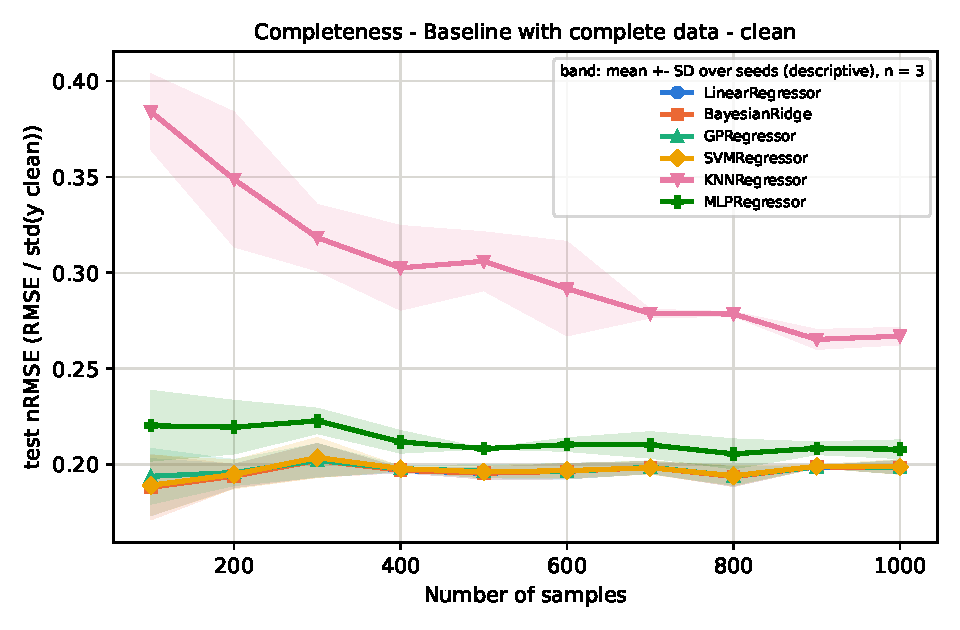
\includegraphics[width=0.8\textwidth]{v3/c00_baseline/clean_test_nrmse.pdf}
\caption{C0: test nRMSE of each model, condition \texttt{clean}, mean $\pm$ SD over 3 seeds.}
\label{fig:c00_baseline_clean_test_nrmse}
\end{figure}

\begin{table}[htbp]
\centering
\small
\resizebox{\textwidth}{!}{% Generated by Report/tools/build_v3_assets.py from Plot/v3/results/c00_baseline.json (metric test_nrmse); do not edit by hand.
% Cells are mean $\pm$ SD over seeds (folds averaged within seed); the band is descriptive, not a confidence interval.
\begin{tabular}{llrrr}
\hline
Condition & Model & 100 & 600 & 1000 \\
\hline
clean & LinearRegressor & 0.188 $\pm$ 0.015 & 0.197 $\pm$ 0.004 & 0.199 $\pm$ 0.004 \\
clean & GPRegressor & 0.194 $\pm$ 0.015 & 0.196 $\pm$ 0.004 & 0.199 $\pm$ 0.004 \\
clean & KNNRegressor & 0.384 $\pm$ 0.020 & 0.292 $\pm$ 0.025 & 0.267 $\pm$ 0.005 \\
clean & MLPRegressor & 0.220 $\pm$ 0.018 & 0.210 $\pm$ 0.004 & 0.208 $\pm$ 0.005 \\
\hline
\end{tabular}
}
\caption{C0: test nRMSE (lower is better) against sample size $n$ (100, 600, 1000 shown); mean $\pm$ SD over 3 seeds.}
\label{tab:c00_baseline}
\end{table}

\subsection{C1: MCAR with low percentages}
\label{sec:c01_mcar_low}
Cells of all 3 informative features are removed completely at random (1000 rows). With 2.5\% missing cells the mean-imputed linear model already moves from $0.199$ (clean) to $0.256 \pm 0.008$, and reaches $0.543 \pm 0.017$ at 25\%. \texttt{median}, \texttt{iterative} and \texttt{mean\_indicator} give practically the same numbers as \texttt{mean} ($0.256$, $0.256$ and $0.254$ at 2.5\%; $0.543$, $0.544$ and $0.541$ at 25\%): the three features are generated independently, so the other columns carry no information on the missing one and every reasonable imputer ends at the column centre. \texttt{knn} is slightly worse ($0.264$ and $0.580$). The two naive options are clearly worse: \texttt{most\_frequent}, which is degenerate on continuous data, gives $0.502$ and $0.880$, and \texttt{std\_constant} (the method of the original study) gives $0.302 \pm 0.027$ and $0.659 \pm 0.034$. \texttt{KNeighborsRegressor} shows the same ordering at a higher level ($0.319 \to 0.616$ with \texttt{mean}). The native-NaN \texttt{HistGradientBoostingRegressor} behaves like its mean-imputed counterpart ($0.296$ against $0.305$ at 2.5\%, $0.601$ against $0.599$ at 25\%).

\begin{figure}[htbp]
\centering
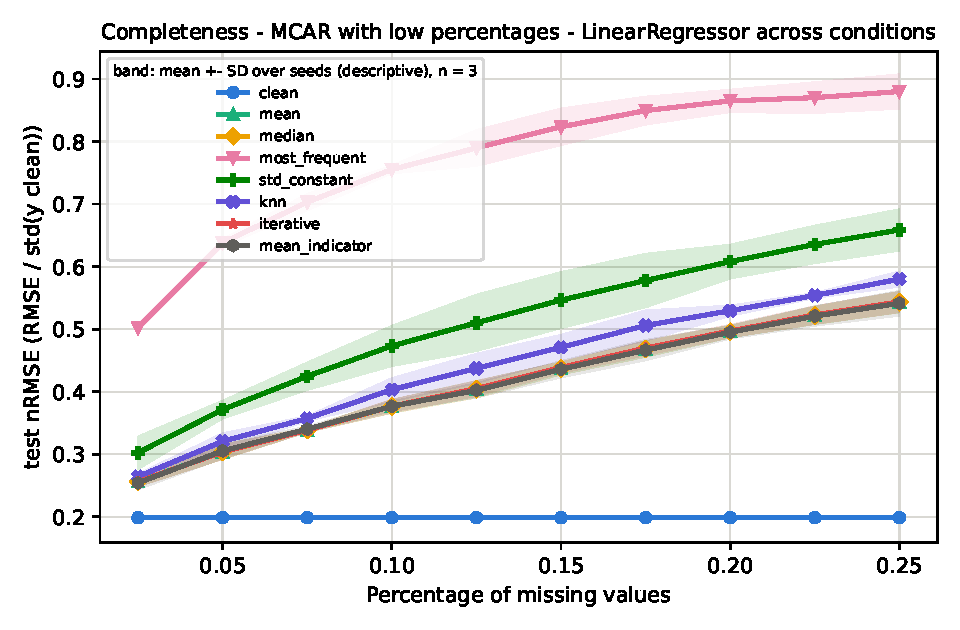
\includegraphics[width=0.8\textwidth]{v3/c01_mcar_low/model_LinearRegressor_test_nrmse.pdf}
\caption{C1: test nRMSE of \texttt{LinearRegressor} for each condition, mean $\pm$ SD over 3 seeds.}
\label{fig:c01_mcar_low_model_LinearRegressor_test_nrmse}
\end{figure}

\begin{figure}[htbp]
\centering
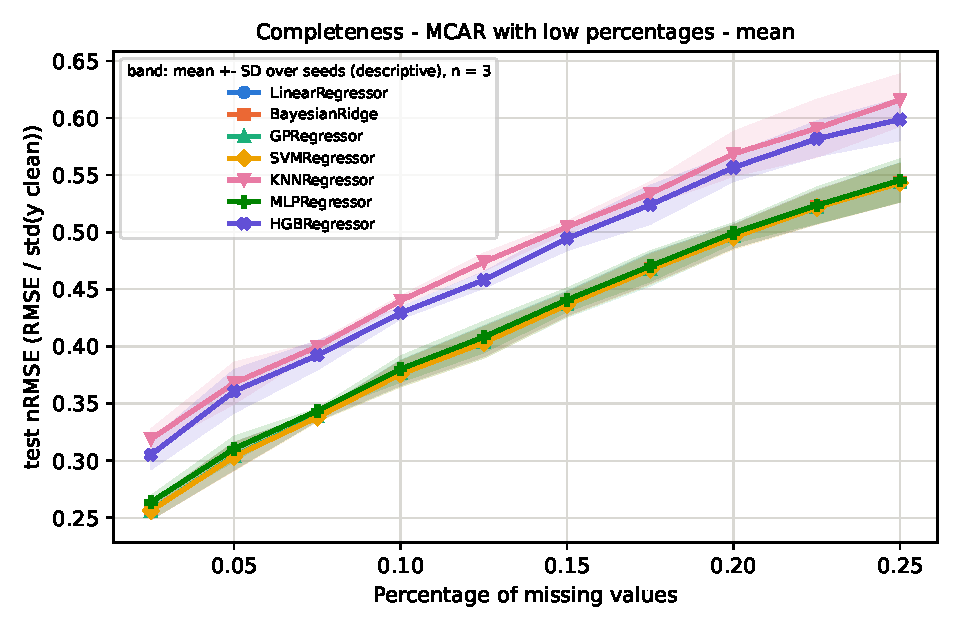
\includegraphics[width=0.8\textwidth]{v3/c01_mcar_low/mean_test_nrmse.pdf}
\caption{C1: test nRMSE of each model, condition \texttt{mean}, mean $\pm$ SD over 3 seeds.}
\label{fig:c01_mcar_low_mean_test_nrmse}
\end{figure}

\begin{figure}[htbp]
\centering
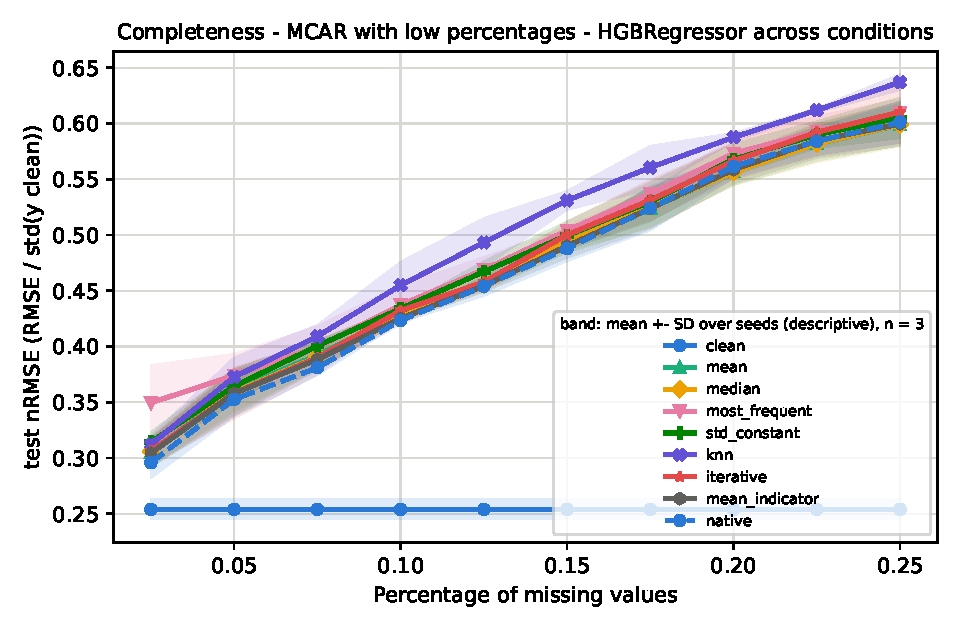
\includegraphics[width=0.8\textwidth]{v3/c01_mcar_low/model_HGBRegressor_test_nrmse.pdf}
\caption{C1: test nRMSE of \texttt{HGBRegressor} for each condition, mean $\pm$ SD over 3 seeds.}
\label{fig:c01_mcar_low_model_HGBRegressor_test_nrmse}
\end{figure}

\begin{table}[htbp]
\centering
\small
\resizebox{\textwidth}{!}{% Generated by Report/tools/build_v3_assets.py from Plot/v3/results/c01_mcar_low.json (metric test_nrmse); do not edit by hand.
% Cells are mean $\pm$ SD over seeds (folds averaged within seed); the band is descriptive, not a confidence interval.
\begin{tabular}{llrrr}
\hline
Condition & Model & 0.025 & 0.15 & 0.25 \\
\hline
clean & LinearRegressor & 0.199 $\pm$ 0.004 & 0.199 $\pm$ 0.004 & 0.199 $\pm$ 0.004 \\
clean & KNNRegressor & 0.267 $\pm$ 0.005 & 0.267 $\pm$ 0.005 & 0.267 $\pm$ 0.005 \\
mean & LinearRegressor & 0.256 $\pm$ 0.008 & 0.437 $\pm$ 0.010 & 0.543 $\pm$ 0.017 \\
mean & KNNRegressor & 0.319 $\pm$ 0.009 & 0.505 $\pm$ 0.005 & 0.616 $\pm$ 0.023 \\
median & LinearRegressor & 0.256 $\pm$ 0.008 & 0.437 $\pm$ 0.010 & 0.543 $\pm$ 0.017 \\
median & KNNRegressor & 0.319 $\pm$ 0.008 & 0.504 $\pm$ 0.008 & 0.614 $\pm$ 0.023 \\
most\_frequent & LinearRegressor & 0.502 $\pm$ 0.007 & 0.824 $\pm$ 0.030 & 0.880 $\pm$ 0.028 \\
most\_frequent & KNNRegressor & 0.375 $\pm$ 0.019 & 0.561 $\pm$ 0.030 & 0.653 $\pm$ 0.038 \\
std\_constant & LinearRegressor & 0.302 $\pm$ 0.027 & 0.546 $\pm$ 0.046 & 0.659 $\pm$ 0.034 \\
std\_constant & KNNRegressor & 0.359 $\pm$ 0.019 & 0.588 $\pm$ 0.029 & 0.683 $\pm$ 0.026 \\
knn & LinearRegressor & 0.264 $\pm$ 0.005 & 0.471 $\pm$ 0.021 & 0.580 $\pm$ 0.013 \\
knn & KNNRegressor & 0.324 $\pm$ 0.005 & 0.531 $\pm$ 0.013 & 0.647 $\pm$ 0.012 \\
iterative & LinearRegressor & 0.256 $\pm$ 0.008 & 0.439 $\pm$ 0.009 & 0.544 $\pm$ 0.017 \\
iterative & KNNRegressor & 0.319 $\pm$ 0.009 & 0.507 $\pm$ 0.005 & 0.616 $\pm$ 0.021 \\
mean\_indicator & LinearRegressor & 0.254 $\pm$ 0.011 & 0.436 $\pm$ 0.014 & 0.541 $\pm$ 0.021 \\
mean\_indicator & KNNRegressor & 0.330 $\pm$ 0.007 & 0.511 $\pm$ 0.016 & 0.619 $\pm$ 0.029 \\
native & HGBRegressor & 0.296 $\pm$ 0.014 & 0.488 $\pm$ 0.012 & 0.601 $\pm$ 0.019 \\
mean & HGBRegressor & 0.305 $\pm$ 0.013 & 0.495 $\pm$ 0.011 & 0.599 $\pm$ 0.019 \\
\hline
\end{tabular}
}
\caption{C1: test nRMSE (lower is better) against missing rate (0.025, 0.15, 0.25 shown); mean $\pm$ SD over 3 seeds.}
\label{tab:c01_mcar_low}
\end{table}

\subsection{C2: MCAR with high percentages}
\label{sec:c02_mcar_high}
The same setting at 27.5\%--50\% missing cells (\texttt{most\_frequent} and \texttt{std\_constant} omitted). The mean-imputed linear model goes from $0.564 \pm 0.011$ to $0.719 \pm 0.006$ and \texttt{KNeighborsRegressor} from $0.634$ to $0.813$. \texttt{knn} imputation is again a little worse ($0.602 \to 0.755$ for the linear model), \texttt{iterative} is equal to \texttt{mean} up to 40\% and slightly worse at 50\% ($0.727$ against $0.719$), and the missing-value indicator brings no gain ($0.718$). The native \texttt{HistGradientBoostingRegressor} gives $0.627 \to 0.780$, close to its mean-imputed version ($0.623 \to 0.774$).

\begin{figure}[htbp]
\centering
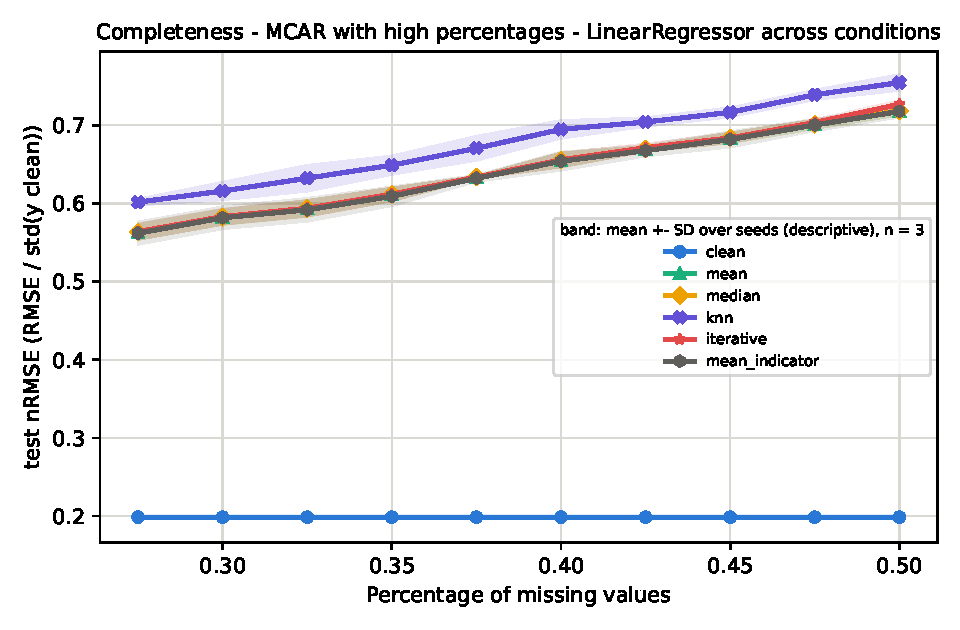
\includegraphics[width=0.8\textwidth]{v3/c02_mcar_high/model_LinearRegressor_test_nrmse.pdf}
\caption{C2: test nRMSE of \texttt{LinearRegressor} for each condition, mean $\pm$ SD over 3 seeds.}
\label{fig:c02_mcar_high_model_LinearRegressor_test_nrmse}
\end{figure}

\begin{figure}[htbp]
\centering
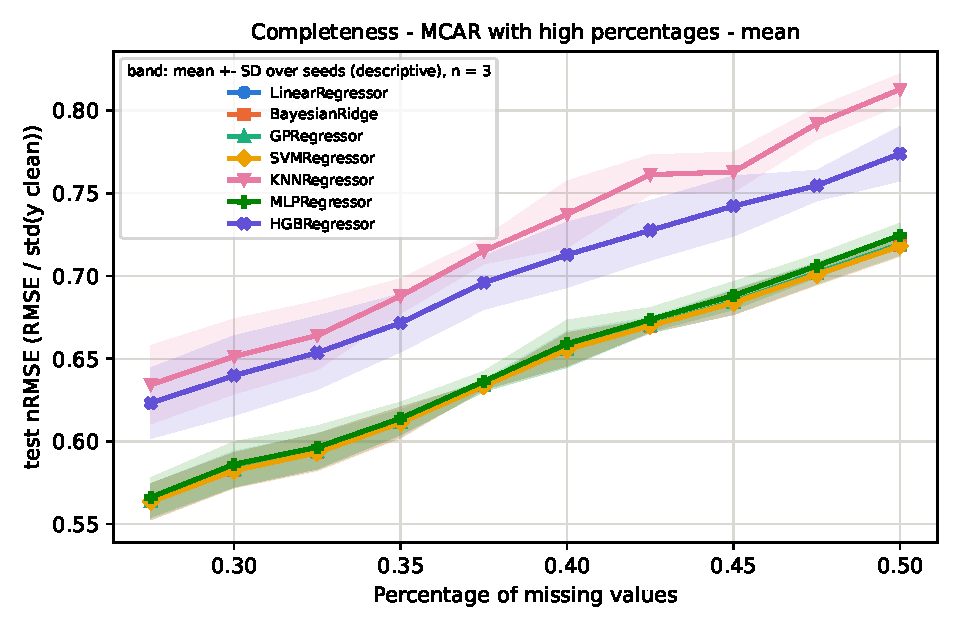
\includegraphics[width=0.8\textwidth]{v3/c02_mcar_high/mean_test_nrmse.pdf}
\caption{C2: test nRMSE of each model, condition \texttt{mean}, mean $\pm$ SD over 3 seeds.}
\label{fig:c02_mcar_high_mean_test_nrmse}
\end{figure}

\begin{figure}[htbp]
\centering
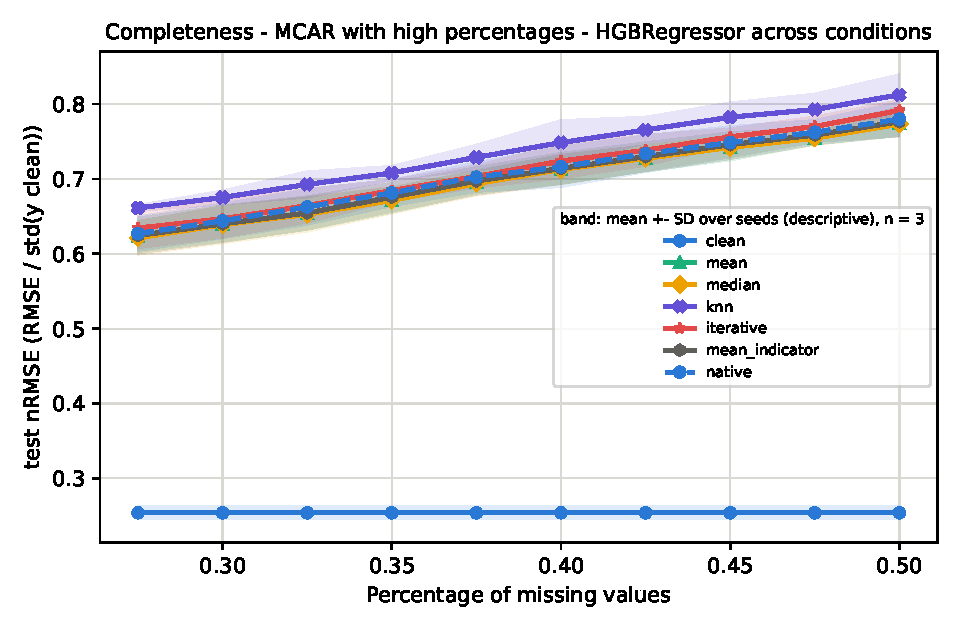
\includegraphics[width=0.8\textwidth]{v3/c02_mcar_high/model_HGBRegressor_test_nrmse.pdf}
\caption{C2: test nRMSE of \texttt{HGBRegressor} for each condition, mean $\pm$ SD over 3 seeds.}
\label{fig:c02_mcar_high_model_HGBRegressor_test_nrmse}
\end{figure}

\begin{table}[htbp]
\centering
\small
\resizebox{\textwidth}{!}{% Generated by Report/tools/build_v3_assets.py from Plot/v3/results/c02_mcar_high.json (metric test_nrmse); do not edit by hand.
% Cells are mean $\pm$ SD over seeds (folds averaged within seed); the band is descriptive, not a confidence interval.
\begin{tabular}{llrrr}
\hline
Condition & Model & 0.275 & 0.4 & 0.5 \\
\hline
clean & LinearRegressor & 0.199 $\pm$ 0.004 & 0.199 $\pm$ 0.004 & 0.199 $\pm$ 0.004 \\
clean & KNNRegressor & 0.267 $\pm$ 0.005 & 0.267 $\pm$ 0.005 & 0.267 $\pm$ 0.005 \\
mean & LinearRegressor & 0.564 $\pm$ 0.011 & 0.656 $\pm$ 0.010 & 0.719 $\pm$ 0.006 \\
mean & KNNRegressor & 0.634 $\pm$ 0.024 & 0.737 $\pm$ 0.020 & 0.813 $\pm$ 0.009 \\
median & LinearRegressor & 0.564 $\pm$ 0.010 & 0.655 $\pm$ 0.010 & 0.719 $\pm$ 0.006 \\
median & KNNRegressor & 0.636 $\pm$ 0.025 & 0.743 $\pm$ 0.014 & 0.803 $\pm$ 0.004 \\
knn & LinearRegressor & 0.602 $\pm$ 0.005 & 0.695 $\pm$ 0.012 & 0.755 $\pm$ 0.011 \\
knn & KNNRegressor & 0.667 $\pm$ 0.018 & 0.757 $\pm$ 0.024 & 0.820 $\pm$ 0.012 \\
iterative & LinearRegressor & 0.564 $\pm$ 0.011 & 0.656 $\pm$ 0.010 & 0.727 $\pm$ 0.006 \\
iterative & KNNRegressor & 0.633 $\pm$ 0.026 & 0.731 $\pm$ 0.020 & 0.797 $\pm$ 0.008 \\
mean\_indicator & LinearRegressor & 0.562 $\pm$ 0.015 & 0.654 $\pm$ 0.013 & 0.718 $\pm$ 0.008 \\
mean\_indicator & KNNRegressor & 0.635 $\pm$ 0.041 & 0.735 $\pm$ 0.020 & 0.808 $\pm$ 0.010 \\
native & HGBRegressor & 0.627 $\pm$ 0.024 & 0.716 $\pm$ 0.028 & 0.780 $\pm$ 0.023 \\
mean & HGBRegressor & 0.623 $\pm$ 0.021 & 0.713 $\pm$ 0.020 & 0.774 $\pm$ 0.017 \\
\hline
\end{tabular}
}
\caption{C2: test nRMSE (lower is better) against missing rate (0.275, 0.4, 0.5 shown); mean $\pm$ SD over 3 seeds.}
\label{tab:c02_mcar_high}
\end{table}

\subsection{C3: fixed MCAR on a single feature}
\label{sec:c03_mcar_one_feature}
20\% of one column is removed; there are 10 features, ranks 0--4 are informative and ranks 5--9 are noise. Missingness in the most important feature (rank 0) raises the mean-imputed linear model from $0.202$ (clean) to $0.365 \pm 0.033$, whereas for the noise features at rank 5 and 9 it stays at $0.202$, identical to the clean value. \texttt{median} and \texttt{iterative} imputation reproduce these values ($0.365$, $0.366$). The native-NaN boosting model shows the same pattern ($0.445$ at rank 0 against $0.301$ and $0.302$ at ranks 5 and 9). Only informative features matter.

\begin{figure}[htbp]
\centering
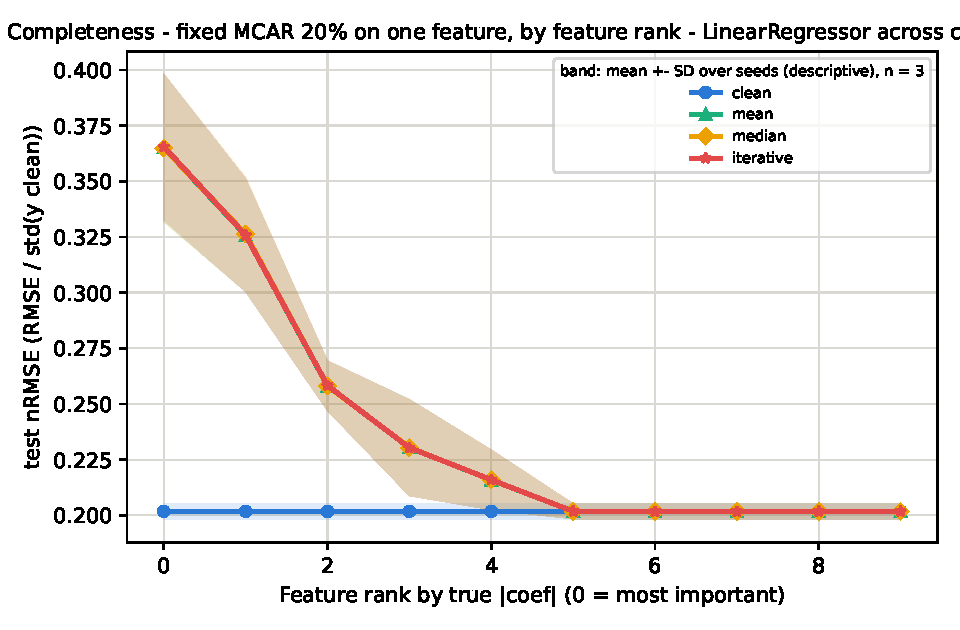
\includegraphics[width=0.8\textwidth]{v3/c03_mcar_one_feature/model_LinearRegressor_test_nrmse.pdf}
\caption{C3: test nRMSE of \texttt{LinearRegressor} for each condition, mean $\pm$ SD over 3 seeds.}
\label{fig:c03_mcar_one_feature_model_LinearRegressor_test_nrmse}
\end{figure}

\begin{table}[htbp]
\centering
\small
\resizebox{\textwidth}{!}{% Generated by Report/tools/build_v3_assets.py from Plot/v3/results/c03_mcar_one_feature.json (metric test_nrmse); do not edit by hand.
% Cells are mean $\pm$ SD over seeds (folds averaged within seed); the band is descriptive, not a confidence interval.
\begin{tabular}{llrrr}
\hline
Condition & Model & 0 & 5 & 9 \\
\hline
clean & LinearRegressor & 0.202 $\pm$ 0.004 & 0.202 $\pm$ 0.004 & 0.202 $\pm$ 0.004 \\
mean & LinearRegressor & 0.365 $\pm$ 0.033 & 0.202 $\pm$ 0.003 & 0.202 $\pm$ 0.004 \\
median & LinearRegressor & 0.365 $\pm$ 0.033 & 0.202 $\pm$ 0.003 & 0.202 $\pm$ 0.004 \\
iterative & LinearRegressor & 0.366 $\pm$ 0.033 & 0.202 $\pm$ 0.003 & 0.202 $\pm$ 0.004 \\
mean & HGBRegressor & 0.446 $\pm$ 0.025 & 0.299 $\pm$ 0.013 & 0.299 $\pm$ 0.014 \\
native & HGBRegressor & 0.445 $\pm$ 0.019 & 0.301 $\pm$ 0.015 & 0.302 $\pm$ 0.013 \\
\hline
\end{tabular}
}
\caption{C3: test nRMSE (lower is better) against feature rank by true $|$coefficient$|$ (0, 5, 9 shown); mean $\pm$ SD over 3 seeds.}
\label{tab:c03_mcar_one_feature}
\end{table}

\subsection{C4: incremental MCAR per feature with growing sample size}
\label{sec:c04_incremental}
Column $i$ loses $10 i$\% of its cells (5 features, 3 informative) while $n$ grows. The linear model with mean imputation gives $0.428 \pm 0.179$, $0.439 \pm 0.152$ and $0.525 \pm 0.097$ at $n=100$, $600$, $1000$, against $0.188$, $0.198$ and $0.200$ for the clean data. There is no reliable trend with $n$ given the SD over seeds, which is large (up to $0.179$). The boosting model shows the same absence of a trend ($0.668$, $0.512$, $0.586$ with \texttt{mean}). The polluter uses the same seed for every column, so the missing-row sets are nested; this is kept and listed as a limitation.

\begin{figure}[htbp]
\centering
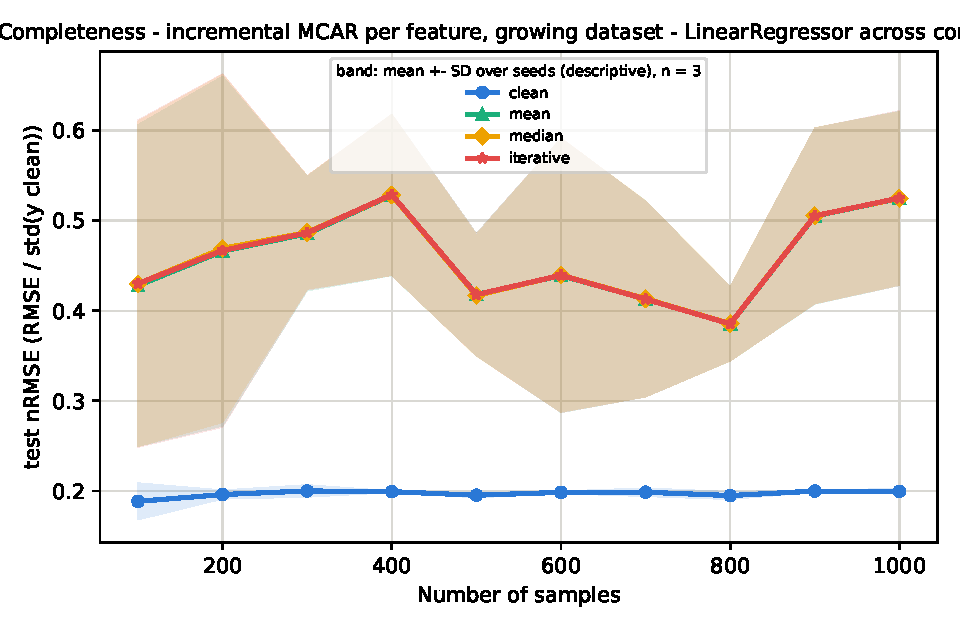
\includegraphics[width=0.8\textwidth]{v3/c04_incremental/model_LinearRegressor_test_nrmse.pdf}
\caption{C4: test nRMSE of \texttt{LinearRegressor} for each condition, mean $\pm$ SD over 3 seeds.}
\label{fig:c04_incremental_model_LinearRegressor_test_nrmse}
\end{figure}

\begin{table}[htbp]
\centering
\small
\resizebox{\textwidth}{!}{% Generated by Report/tools/build_v3_assets.py from Plot/v3/results/c04_incremental.json (metric test_nrmse); do not edit by hand.
% Cells are mean $\pm$ SD over seeds (folds averaged within seed); the band is descriptive, not a confidence interval.
\begin{tabular}{llrrr}
\hline
Condition & Model & 100 & 600 & 1000 \\
\hline
clean & LinearRegressor & 0.188 $\pm$ 0.021 & 0.198 $\pm$ 0.002 & 0.200 $\pm$ 0.003 \\
mean & LinearRegressor & 0.428 $\pm$ 0.179 & 0.439 $\pm$ 0.152 & 0.525 $\pm$ 0.097 \\
median & LinearRegressor & 0.430 $\pm$ 0.181 & 0.439 $\pm$ 0.152 & 0.525 $\pm$ 0.096 \\
iterative & LinearRegressor & 0.430 $\pm$ 0.182 & 0.439 $\pm$ 0.152 & 0.525 $\pm$ 0.097 \\
mean & HGBRegressor & 0.668 $\pm$ 0.170 & 0.512 $\pm$ 0.166 & 0.586 $\pm$ 0.109 \\
native & HGBRegressor & 0.604 $\pm$ 0.140 & 0.506 $\pm$ 0.160 & 0.585 $\pm$ 0.106 \\
\hline
\end{tabular}
}
\caption{C4: test nRMSE (lower is better) against sample size $n$ (100, 600, 1000 shown); mean $\pm$ SD over 3 seeds.}
\label{tab:c04_incremental}
\end{table}

\subsection{C5: MAR}
\label{sec:c05_mar}
Feature 2 is removed where feature 1 exceeds its $(1-x)$ quantile, so the realised rate is $x$ and depends only on an observed value. The effect is mild at the tested rates, but only one column is affected, so this is not a like-for-like comparison with MCAR on all features (C1, C2); the closest one-column reference is C3. The mean-imputed linear model gives $0.217 \pm 0.023$, $0.269 \pm 0.085$ and $0.309 \pm 0.128$ at 5\%, 30\% and 50\% (clean $0.199$). \texttt{median}, \texttt{iterative} and \texttt{mean\_indicator} are indistinguishable from \texttt{mean} (for example $0.309$, $0.309$ and $0.310$ at 50\%). The SD over seeds grows with the rate, so the seeds disagree on how harmful the mechanism is. Native boosting gives $0.263$, $0.320$, $0.362$.

\begin{figure}[htbp]
\centering
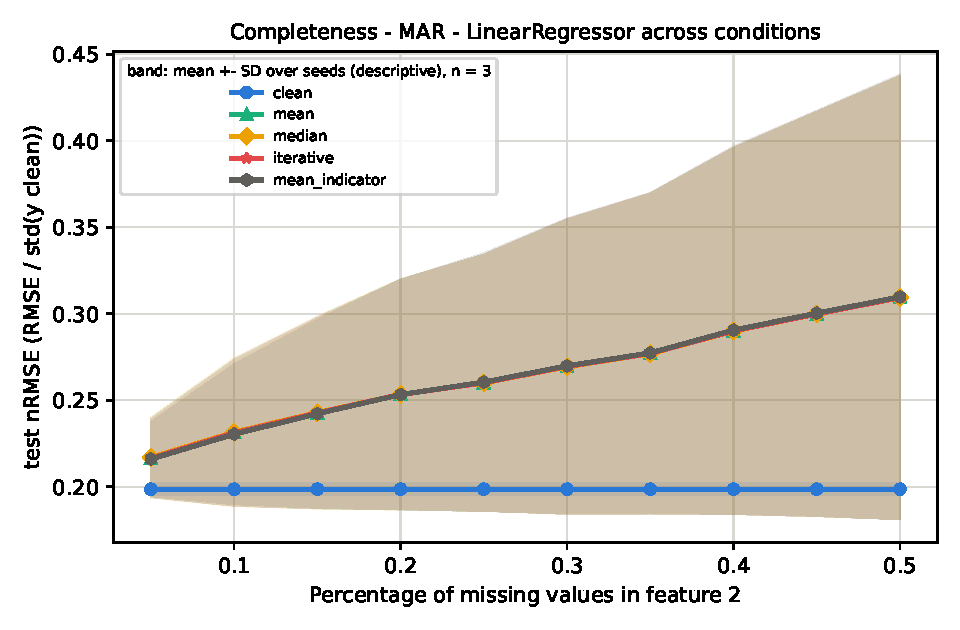
\includegraphics[width=0.8\textwidth]{v3/c05_mar/model_LinearRegressor_test_nrmse.pdf}
\caption{C5: test nRMSE of \texttt{LinearRegressor} for each condition, mean $\pm$ SD over 3 seeds.}
\label{fig:c05_mar_model_LinearRegressor_test_nrmse}
\end{figure}

\begin{table}[htbp]
\centering
\small
\resizebox{\textwidth}{!}{% Generated by Report/tools/build_v3_assets.py from Plot/v3/results/c05_mar.json (metric test_nrmse); do not edit by hand.
% Cells are mean $\pm$ SD over seeds (folds averaged within seed); the band is descriptive, not a confidence interval.
\begin{tabular}{llrrr}
\hline
Condition & Model & 0.05 & 0.3 & 0.5 \\
\hline
clean & LinearRegressor & 0.199 $\pm$ 0.004 & 0.199 $\pm$ 0.004 & 0.199 $\pm$ 0.004 \\
mean & LinearRegressor & 0.217 $\pm$ 0.023 & 0.269 $\pm$ 0.085 & 0.309 $\pm$ 0.128 \\
median & LinearRegressor & 0.217 $\pm$ 0.023 & 0.269 $\pm$ 0.085 & 0.309 $\pm$ 0.128 \\
iterative & LinearRegressor & 0.216 $\pm$ 0.023 & 0.269 $\pm$ 0.086 & 0.309 $\pm$ 0.128 \\
mean\_indicator & LinearRegressor & 0.216 $\pm$ 0.022 & 0.270 $\pm$ 0.086 & 0.310 $\pm$ 0.129 \\
mean & HGBRegressor & 0.265 $\pm$ 0.024 & 0.320 $\pm$ 0.093 & 0.363 $\pm$ 0.139 \\
native & HGBRegressor & 0.263 $\pm$ 0.023 & 0.320 $\pm$ 0.090 & 0.362 $\pm$ 0.138 \\
\hline
\end{tabular}
}
\caption{C5: test nRMSE (lower is better) against missing rate (0.05, 0.3, 0.5 shown); mean $\pm$ SD over 3 seeds.}
\label{tab:c05_mar}
\end{table}

\subsection{C6: MNAR upper tail (self-masking)}
\label{sec:c06_mnar}
Feature 1 is removed when its own value exceeds its $(1-x)$ quantile, so the largest values vanish. Here the imputer matters. Mean imputation of the linear model gives $0.422 \pm 0.048$, $0.664 \pm 0.092$ and $0.740 \pm 0.112$, and \texttt{iterative} imputation is identical ($0.422$, $0.664$, $0.740$): both place the missing values at the centre of the observed (truncated) distribution and are biased. Adding the missing-value indicator recovers a large part of the loss ($0.206 \pm 0.003$, $0.301 \pm 0.024$, $0.388 \pm 0.041$), because the indicator tells the model that the value was in the upper tail. The native boosting model behaves like the indicator variant ($0.257$, $0.350$, $0.443$) and is better than its mean-imputed version at 5\% ($0.292$) but similar at 30\% and 50\% ($0.358$, $0.452$), within one SD.

\begin{figure}[htbp]
\centering
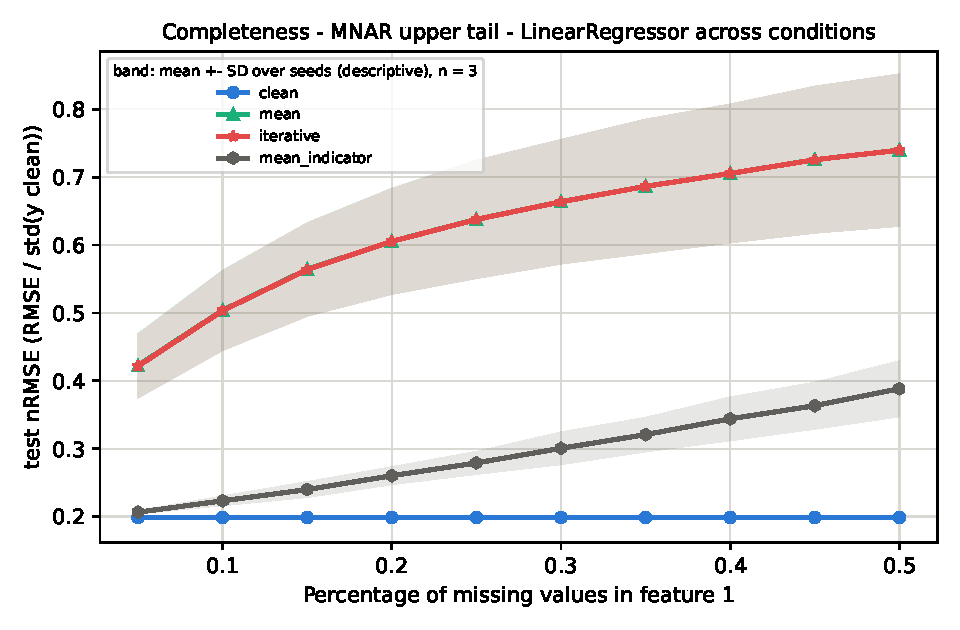
\includegraphics[width=0.8\textwidth]{v3/c06_mnar/model_LinearRegressor_test_nrmse.pdf}
\caption{C6: test nRMSE of \texttt{LinearRegressor} for each condition, mean $\pm$ SD over 3 seeds.}
\label{fig:c06_mnar_model_LinearRegressor_test_nrmse}
\end{figure}

\begin{figure}[htbp]
\centering
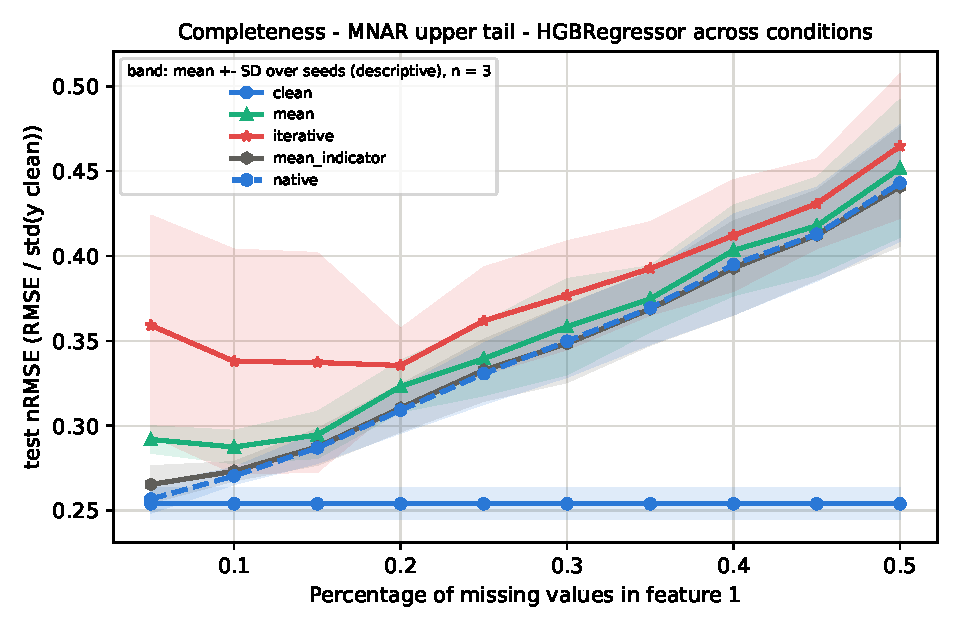
\includegraphics[width=0.8\textwidth]{v3/c06_mnar/model_HGBRegressor_test_nrmse.pdf}
\caption{C6: test nRMSE of \texttt{HGBRegressor} for each condition, mean $\pm$ SD over 3 seeds.}
\label{fig:c06_mnar_model_HGBRegressor_test_nrmse}
\end{figure}

\begin{table}[htbp]
\centering
\small
\resizebox{\textwidth}{!}{% Generated by Report/tools/build_v3_assets.py from Plot/v3/results/c06_mnar.json (metric test_nrmse); do not edit by hand.
% Cells are mean $\pm$ SD over seeds (folds averaged within seed); the band is descriptive, not a confidence interval.
\begin{tabular}{llrrr}
\hline
Condition & Model & 0.05 & 0.3 & 0.5 \\
\hline
clean & LinearRegressor & 0.199 $\pm$ 0.004 & 0.199 $\pm$ 0.004 & 0.199 $\pm$ 0.004 \\
mean & LinearRegressor & 0.422 $\pm$ 0.048 & 0.664 $\pm$ 0.092 & 0.740 $\pm$ 0.112 \\
iterative & LinearRegressor & 0.422 $\pm$ 0.047 & 0.664 $\pm$ 0.092 & 0.740 $\pm$ 0.112 \\
mean\_indicator & LinearRegressor & 0.206 $\pm$ 0.003 & 0.301 $\pm$ 0.024 & 0.388 $\pm$ 0.041 \\
mean & HGBRegressor & 0.292 $\pm$ 0.008 & 0.358 $\pm$ 0.028 & 0.452 $\pm$ 0.041 \\
mean\_indicator & HGBRegressor & 0.265 $\pm$ 0.011 & 0.348 $\pm$ 0.023 & 0.441 $\pm$ 0.035 \\
native & HGBRegressor & 0.257 $\pm$ 0.008 & 0.350 $\pm$ 0.021 & 0.443 $\pm$ 0.034 \\
\hline
\end{tabular}
}
\caption{C6: test nRMSE (lower is better) against missing rate (0.05, 0.3, 0.5 shown); mean $\pm$ SD over 3 seeds.}
\label{tab:c06_mnar}
\end{table}

\subsection{C7: MCAR in the most informative features}
\label{sec:c07_mcar_most}
The 3 most important of 9 features (4 informative) lose 5\%--50\% of their cells. The mean-imputed linear model gives $0.300 \pm 0.021$, $0.578 \pm 0.038$ and $0.705 \pm 0.035$ (clean $0.200$); \texttt{median} and \texttt{iterative} are equal. Native boosting is slightly worse ($0.373$, $0.647$, $0.792$).

\begin{figure}[htbp]
\centering
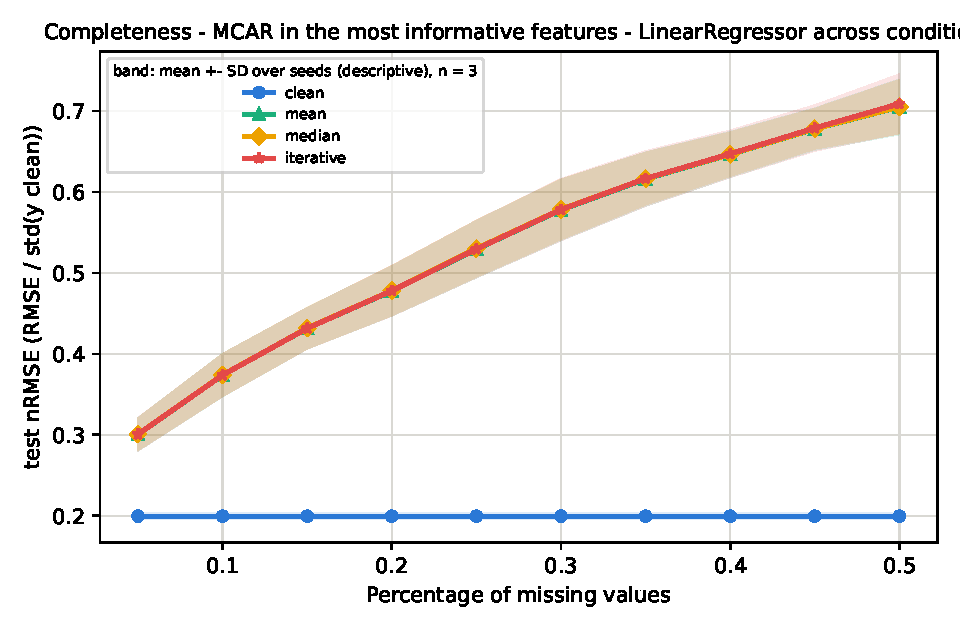
\includegraphics[width=0.8\textwidth]{v3/c07_mcar_most/model_LinearRegressor_test_nrmse.pdf}
\caption{C7: test nRMSE of \texttt{LinearRegressor} for each condition, mean $\pm$ SD over 3 seeds.}
\label{fig:c07_mcar_most_model_LinearRegressor_test_nrmse}
\end{figure}

\begin{table}[htbp]
\centering
\small
\resizebox{\textwidth}{!}{% Generated by Report/tools/build_v3_assets.py from Plot/v3/results/c07_mcar_most.json (metric test_nrmse); do not edit by hand.
% Cells are mean $\pm$ SD over seeds (folds averaged within seed); the band is descriptive, not a confidence interval.
\begin{tabular}{llrrr}
\hline
Condition & Model & 0.05 & 0.3 & 0.5 \\
\hline
clean & LinearRegressor & 0.200 $\pm$ 0.005 & 0.200 $\pm$ 0.005 & 0.200 $\pm$ 0.005 \\
mean & LinearRegressor & 0.300 $\pm$ 0.021 & 0.578 $\pm$ 0.038 & 0.705 $\pm$ 0.035 \\
median & LinearRegressor & 0.301 $\pm$ 0.020 & 0.578 $\pm$ 0.037 & 0.705 $\pm$ 0.034 \\
iterative & LinearRegressor & 0.301 $\pm$ 0.021 & 0.578 $\pm$ 0.039 & 0.709 $\pm$ 0.037 \\
mean & HGBRegressor & 0.372 $\pm$ 0.014 & 0.651 $\pm$ 0.053 & 0.796 $\pm$ 0.027 \\
native & HGBRegressor & 0.373 $\pm$ 0.019 & 0.647 $\pm$ 0.051 & 0.792 $\pm$ 0.029 \\
\hline
\end{tabular}
}
\caption{C7: test nRMSE (lower is better) against missing rate (0.05, 0.3, 0.5 shown); mean $\pm$ SD over 3 seeds.}
\label{tab:c07_mcar_most}
\end{table}

\subsection{C8: MCAR in the less informative features}
\label{sec:c08_mcar_less}
The same experiment for the 3 least important features. The linear model with any imputer stays at $0.199$ for all rates, the clean value, and boosting stays at about $0.27$ ($0.270$, $0.269$, $0.268$ with \texttt{mean}). Missing values in uninformative columns are harmless.

\begin{figure}[htbp]
\centering
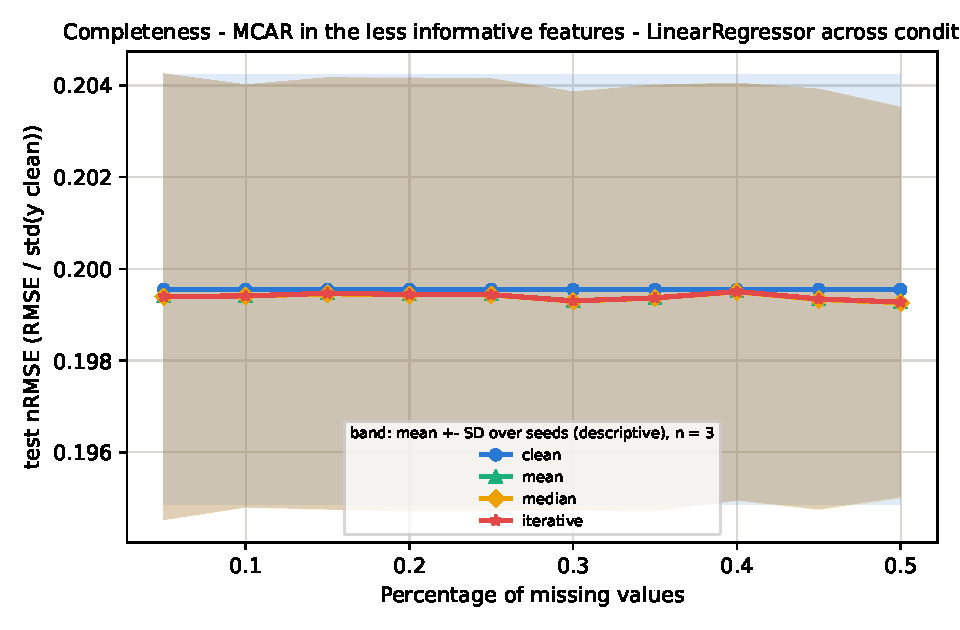
\includegraphics[width=0.8\textwidth]{v3/c08_mcar_less/model_LinearRegressor_test_nrmse.pdf}
\caption{C8: test nRMSE of \texttt{LinearRegressor} for each condition, mean $\pm$ SD over 3 seeds.}
\label{fig:c08_mcar_less_model_LinearRegressor_test_nrmse}
\end{figure}

\begin{table}[htbp]
\centering
\small
\resizebox{\textwidth}{!}{% Generated by Report/tools/build_v3_assets.py from Plot/v3/results/c08_mcar_less.json (metric test_nrmse); do not edit by hand.
% Cells are mean $\pm$ SD over seeds (folds averaged within seed); the band is descriptive, not a confidence interval.
\begin{tabular}{llrrr}
\hline
Condition & Model & 0.05 & 0.3 & 0.5 \\
\hline
clean & LinearRegressor & 0.200 $\pm$ 0.005 & 0.200 $\pm$ 0.005 & 0.200 $\pm$ 0.005 \\
mean & LinearRegressor & 0.199 $\pm$ 0.005 & 0.199 $\pm$ 0.005 & 0.199 $\pm$ 0.004 \\
median & LinearRegressor & 0.199 $\pm$ 0.005 & 0.199 $\pm$ 0.005 & 0.199 $\pm$ 0.004 \\
iterative & LinearRegressor & 0.199 $\pm$ 0.005 & 0.199 $\pm$ 0.005 & 0.199 $\pm$ 0.004 \\
mean & HGBRegressor & 0.270 $\pm$ 0.008 & 0.269 $\pm$ 0.007 & 0.268 $\pm$ 0.008 \\
native & HGBRegressor & 0.271 $\pm$ 0.010 & 0.272 $\pm$ 0.008 & 0.269 $\pm$ 0.007 \\
\hline
\end{tabular}
}
\caption{C8: test nRMSE (lower is better) against missing rate (0.05, 0.3, 0.5 shown); mean $\pm$ SD over 3 seeds.}
\label{tab:c08_mcar_less}
\end{table}

\subsection{C9: MCAR mixing informative and non-informative features}
\label{sec:c09_mcar_mixed}
Both sets (the 3 most and the 3 least important features, ranked once on the clean data) lose cells. The numbers coincide with C7 ($0.301$, $0.577$, $0.705$ for the mean-imputed linear model), showing that the additional uninformative columns add nothing. Boosting with \texttt{mean} gives $0.372$, $0.654$, $0.801$. Because the groups of C7 and C9 share row sets, the two experiments are not independent evidence.

\begin{figure}[htbp]
\centering
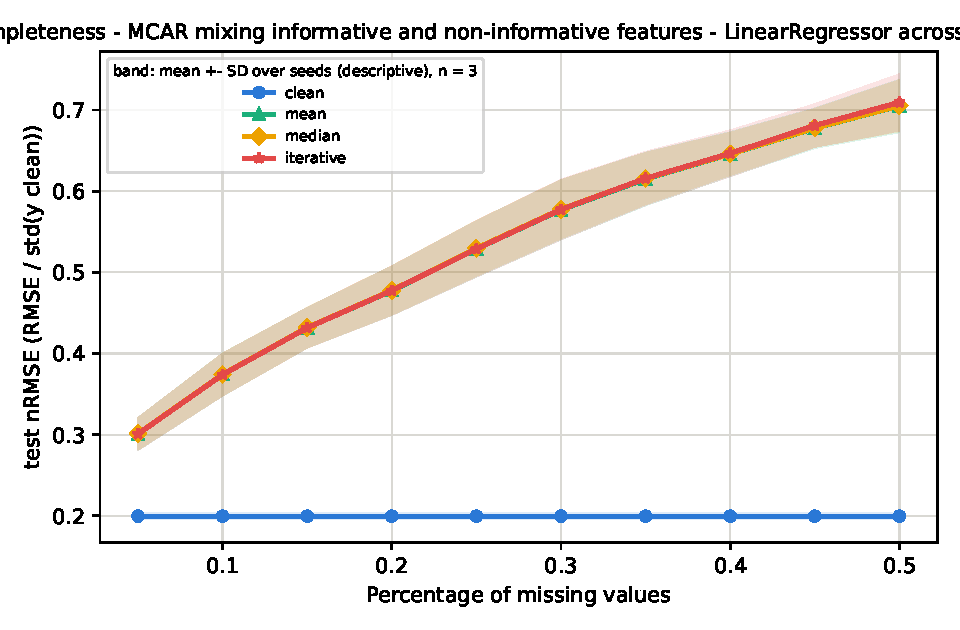
\includegraphics[width=0.8\textwidth]{v3/c09_mcar_mixed/model_LinearRegressor_test_nrmse.pdf}
\caption{C9: test nRMSE of \texttt{LinearRegressor} for each condition, mean $\pm$ SD over 3 seeds.}
\label{fig:c09_mcar_mixed_model_LinearRegressor_test_nrmse}
\end{figure}

\begin{table}[htbp]
\centering
\small
\resizebox{\textwidth}{!}{% Generated by Report/tools/build_v3_assets.py from Plot/v3/results/c09_mcar_mixed.json (metric test_nrmse); do not edit by hand.
% Cells are mean $\pm$ SD over seeds (folds averaged within seed); the band is descriptive, not a confidence interval.
\begin{tabular}{llrrr}
\hline
Condition & Model & 0.05 & 0.3 & 0.5 \\
\hline
clean & LinearRegressor & 0.200 $\pm$ 0.005 & 0.200 $\pm$ 0.005 & 0.200 $\pm$ 0.005 \\
mean & LinearRegressor & 0.301 $\pm$ 0.020 & 0.577 $\pm$ 0.037 & 0.705 $\pm$ 0.033 \\
median & LinearRegressor & 0.301 $\pm$ 0.020 & 0.578 $\pm$ 0.036 & 0.705 $\pm$ 0.032 \\
iterative & LinearRegressor & 0.301 $\pm$ 0.020 & 0.577 $\pm$ 0.037 & 0.709 $\pm$ 0.035 \\
mean & HGBRegressor & 0.372 $\pm$ 0.016 & 0.654 $\pm$ 0.051 & 0.801 $\pm$ 0.032 \\
native & HGBRegressor & 0.377 $\pm$ 0.022 & 0.659 $\pm$ 0.046 & 0.807 $\pm$ 0.035 \\
\hline
\end{tabular}
}
\caption{C9: test nRMSE (lower is better) against missing rate (0.05, 0.3, 0.5 shown); mean $\pm$ SD over 3 seeds.}
\label{tab:c09_mcar_mixed}
\end{table}

\subsection{C10: MCAR on all features combined with MNAR on one feature}
\label{sec:c10_mcar_mnar}
All 10 features lose a share $x$ of their cells at random and feature 0 additionally loses its upper-tail 25\%. The mean-imputed linear model gives $0.346 \pm 0.042$, $0.595 \pm 0.032$, $0.748 \pm 0.012$. The indicator helps at 5\% ($0.310 \pm 0.014$) but not at higher rates ($0.589$ at 30\%, $0.749$ at 50\%), presumably because the MCAR component dominates. Note that feature 0 has a realised missing rate of about $0.25+0.75x$ ($0.29$ at 5\%, $0.63$ at 50\%), so the rate axis is not the missing rate of feature 0. \texttt{iterative} imputation is clearly worse at 50\% ($0.877 \pm 0.020$). Boosting is similar to mean imputation with native NaN handling ($0.435$, $0.687$, $0.841$).

\begin{figure}[htbp]
\centering
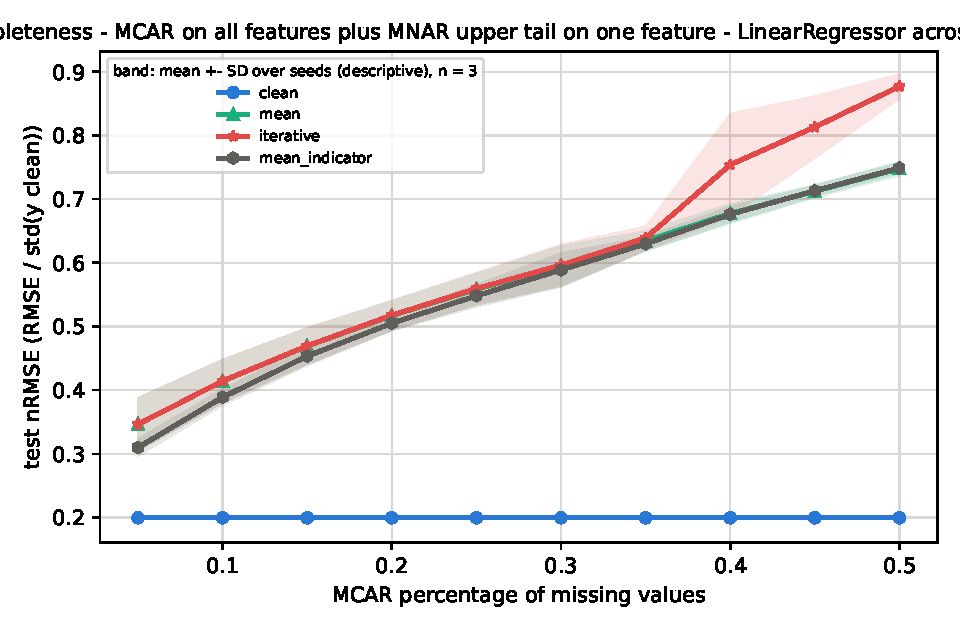
\includegraphics[width=0.8\textwidth]{v3/c10_mcar_mnar/model_LinearRegressor_test_nrmse.pdf}
\caption{C10: test nRMSE of \texttt{LinearRegressor} for each condition, mean $\pm$ SD over 3 seeds.}
\label{fig:c10_mcar_mnar_model_LinearRegressor_test_nrmse}
\end{figure}

\begin{figure}[htbp]
\centering
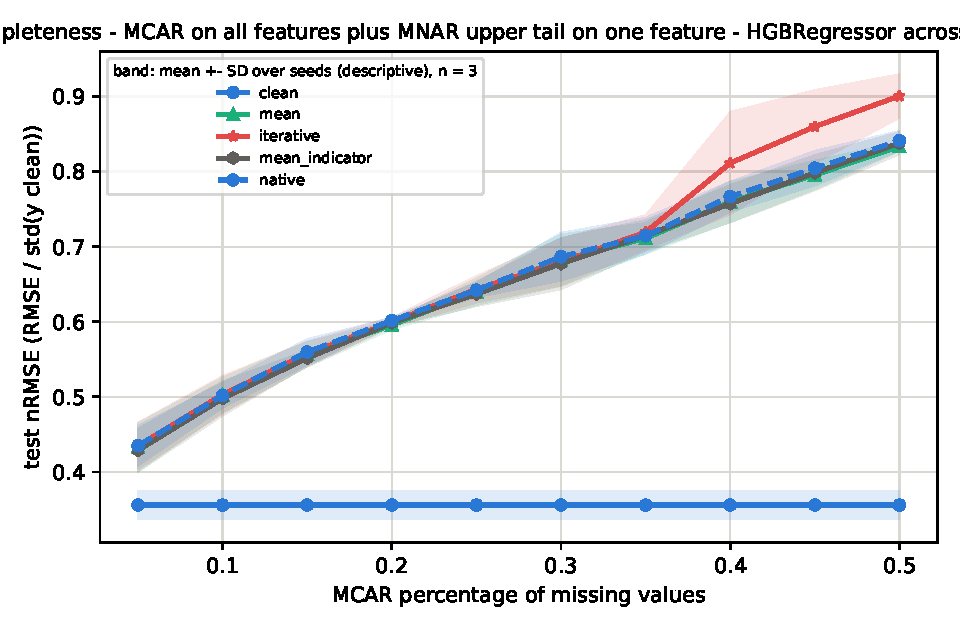
\includegraphics[width=0.8\textwidth]{v3/c10_mcar_mnar/model_HGBRegressor_test_nrmse.pdf}
\caption{C10: test nRMSE of \texttt{HGBRegressor} for each condition, mean $\pm$ SD over 3 seeds.}
\label{fig:c10_mcar_mnar_model_HGBRegressor_test_nrmse}
\end{figure}

\begin{table}[htbp]
\centering
\small
\resizebox{\textwidth}{!}{% Generated by Report/tools/build_v3_assets.py from Plot/v3/results/c10_mcar_mnar.json (metric test_nrmse); do not edit by hand.
% Cells are mean $\pm$ SD over seeds (folds averaged within seed); the band is descriptive, not a confidence interval.
\begin{tabular}{llrrr}
\hline
Condition & Model & 0.05 & 0.3 & 0.5 \\
\hline
clean & LinearRegressor & 0.200 $\pm$ 0.003 & 0.200 $\pm$ 0.003 & 0.200 $\pm$ 0.003 \\
mean & LinearRegressor & 0.346 $\pm$ 0.042 & 0.595 $\pm$ 0.032 & 0.748 $\pm$ 0.012 \\
iterative & LinearRegressor & 0.346 $\pm$ 0.042 & 0.596 $\pm$ 0.033 & 0.877 $\pm$ 0.020 \\
mean\_indicator & LinearRegressor & 0.310 $\pm$ 0.014 & 0.589 $\pm$ 0.027 & 0.749 $\pm$ 0.009 \\
mean & HGBRegressor & 0.433 $\pm$ 0.033 & 0.682 $\pm$ 0.035 & 0.833 $\pm$ 0.006 \\
mean\_indicator & HGBRegressor & 0.429 $\pm$ 0.029 & 0.677 $\pm$ 0.035 & 0.838 $\pm$ 0.015 \\
native & HGBRegressor & 0.435 $\pm$ 0.027 & 0.687 $\pm$ 0.033 & 0.841 $\pm$ 0.014 \\
\hline
\end{tabular}
}
\caption{C10: test nRMSE (lower is better) against MCAR rate (0.05, 0.3, 0.5 shown); mean $\pm$ SD over 3 seeds.}
\label{tab:c10_mcar_mnar}
\end{table}

\section{Distinctness}
\label{sec:res_distinctness}%
\subsection*{Family A: feature-value distinctness}
\subsection{D1: mid-high distinctness}
\label{sec:d1_mid_high}
One random feature of 3 loses distinct values. The polluted linear model rises from $0.199$ to $0.240 \pm 0.020$ at 25\% and $0.271 \pm 0.038$ at 50\%, and the other models follow the same curve (BayesianRidge $0.271$, Gaussian process $0.271$, \texttt{KNeighborsRegressor} $0.267 \to 0.333$). The pollution pastes another row's value into a cell, so it is also a value-substitution (accuracy) error.

\begin{figure}[htbp]
\centering
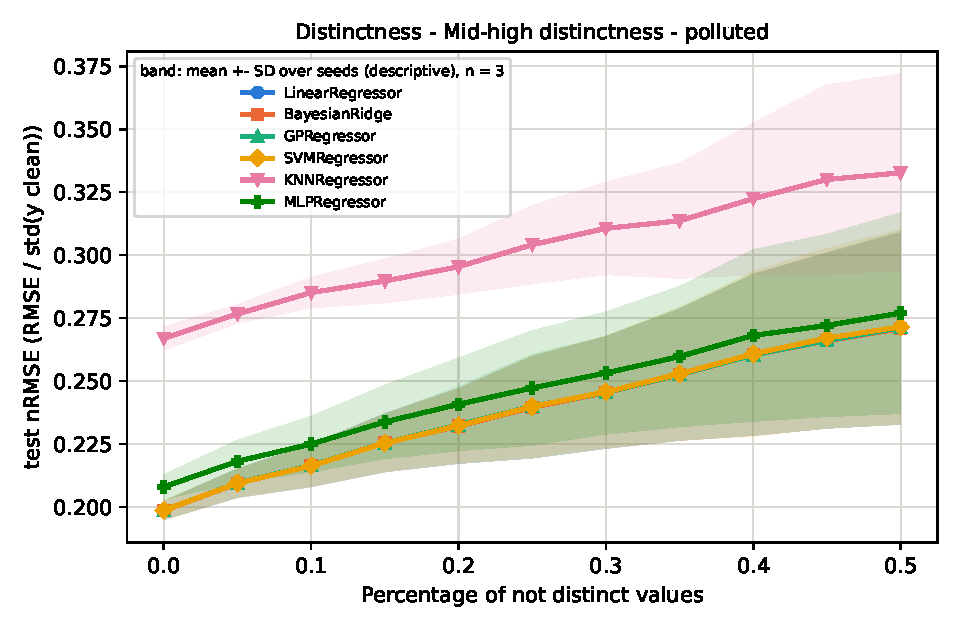
\includegraphics[width=0.8\textwidth]{v3/d1_mid_high/polluted_test_nrmse.pdf}
\caption{D1: test nRMSE of each model, condition \texttt{polluted}, mean $\pm$ SD over 3 seeds.}
\label{fig:d1_mid_high_polluted_test_nrmse}
\end{figure}

\begin{table}[htbp]
\centering
\small
\resizebox{\textwidth}{!}{% Generated by Report/tools/build_v3_assets.py from Plot/v3/results/d1_mid_high.json (metric test_nrmse); do not edit by hand.
% Cells are mean $\pm$ SD over seeds (folds averaged within seed); the band is descriptive, not a confidence interval.
\begin{tabular}{llrrr}
\hline
Condition & Model & 0 & 0.25 & 0.5 \\
\hline
polluted & LinearRegressor & 0.199 $\pm$ 0.004 & 0.240 $\pm$ 0.020 & 0.271 $\pm$ 0.038 \\
polluted & BayesianRidge & 0.199 $\pm$ 0.004 & 0.240 $\pm$ 0.020 & 0.271 $\pm$ 0.038 \\
polluted & GPRegressor & 0.199 $\pm$ 0.004 & 0.240 $\pm$ 0.021 & 0.271 $\pm$ 0.038 \\
polluted & SVMRegressor & 0.199 $\pm$ 0.004 & 0.240 $\pm$ 0.020 & 0.272 $\pm$ 0.039 \\
polluted & KNNRegressor & 0.267 $\pm$ 0.005 & 0.304 $\pm$ 0.016 & 0.333 $\pm$ 0.039 \\
polluted & MLPRegressor & 0.208 $\pm$ 0.005 & 0.247 $\pm$ 0.023 & 0.277 $\pm$ 0.040 \\
clean & LinearRegressor & 0.199 $\pm$ 0.004 & 0.199 $\pm$ 0.004 & 0.199 $\pm$ 0.004 \\
\hline
\end{tabular}
}
\caption{D1: test nRMSE (lower is better) against fraction of non-distinct values (0, 0.25, 0.5 shown); mean $\pm$ SD over 3 seeds.}
\label{tab:d1_mid_high}
\end{table}

\subsection{D2: mid-low distinctness}
\label{sec:d2_mid_low}
From 50\% to 100\% the linear model goes $0.271 \pm 0.038$, $0.282 \pm 0.045$, $0.282 \pm 0.045$: the curve saturates, and at 100\% the column is constant, so the models effectively lose one feature. The difference between seeds ($\pm 0.045$) presumably reflects which random feature was polluted.

\begin{figure}[htbp]
\centering
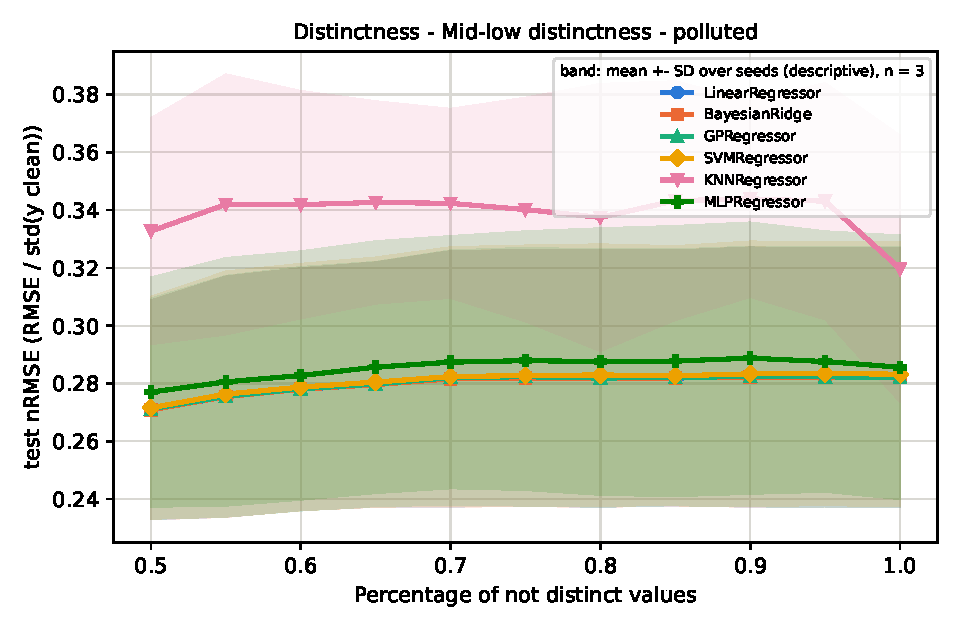
\includegraphics[width=0.8\textwidth]{v3/d2_mid_low/polluted_test_nrmse.pdf}
\caption{D2: test nRMSE of each model, condition \texttt{polluted}, mean $\pm$ SD over 3 seeds.}
\label{fig:d2_mid_low_polluted_test_nrmse}
\end{figure}

\begin{table}[htbp]
\centering
\small
\resizebox{\textwidth}{!}{% Generated by Report/tools/build_v3_assets.py from Plot/v3/results/d2_mid_low.json (metric test_nrmse); do not edit by hand.
% Cells are mean $\pm$ SD over seeds (folds averaged within seed); the band is descriptive, not a confidence interval.
\begin{tabular}{llrrr}
\hline
Condition & Model & 0.5 & 0.75 & 1 \\
\hline
polluted & LinearRegressor & 0.271 $\pm$ 0.038 & 0.282 $\pm$ 0.045 & 0.282 $\pm$ 0.045 \\
polluted & BayesianRidge & 0.271 $\pm$ 0.038 & 0.282 $\pm$ 0.045 & 0.282 $\pm$ 0.045 \\
polluted & GPRegressor & 0.271 $\pm$ 0.038 & 0.282 $\pm$ 0.045 & 0.282 $\pm$ 0.045 \\
polluted & SVMRegressor & 0.272 $\pm$ 0.039 & 0.283 $\pm$ 0.045 & 0.283 $\pm$ 0.046 \\
polluted & KNNRegressor & 0.333 $\pm$ 0.039 & 0.340 $\pm$ 0.039 & 0.320 $\pm$ 0.046 \\
polluted & MLPRegressor & 0.277 $\pm$ 0.040 & 0.288 $\pm$ 0.045 & 0.286 $\pm$ 0.046 \\
clean & LinearRegressor & 0.199 $\pm$ 0.004 & 0.199 $\pm$ 0.004 & 0.199 $\pm$ 0.004 \\
\hline
\end{tabular}
}
\caption{D2: test nRMSE (lower is better) against fraction of non-distinct values (0.5, 0.75, 1 shown); mean $\pm$ SD over 3 seeds.}
\label{tab:d2_mid_low}
\end{table}

\subsection{D3: fixed distinctness, increasing sample size}
\label{sec:d3_fixed_n}
With a fixed 20\% of non-distinct values in one random feature, the linear model gives $0.412 \pm 0.102$, $0.514 \pm 0.052$ and $0.232 \pm 0.015$ at $n=100$, 600 and 1000 (clean $0.188$, $0.197$, $0.199$). There is no monotone size trend, and the variation is mainly between the values of $n$ rather than between seeds (the SD over seeds is moderate and falls with $n$). In this experiment the data are regenerated for each $n$ (\texttt{make\_data(seed, x)}). Within a seed, the polluter (\texttt{pollution\_first\_second\_third\_experiments} in \texttt{library/v2/my\_functions.py}, seeded with the per-repetition pollute seed) picks the same column index at every $n$, but \texttt{make\_regression} draws the coefficients after $X$, so the true coefficients, and hence the weight of the polluted column, change with $n$. The curve therefore reflects the weight of the polluted feature at each $n$, not the sample size. The realised distinct fraction is $0.8$ at every $n$.

\begin{figure}[htbp]
\centering
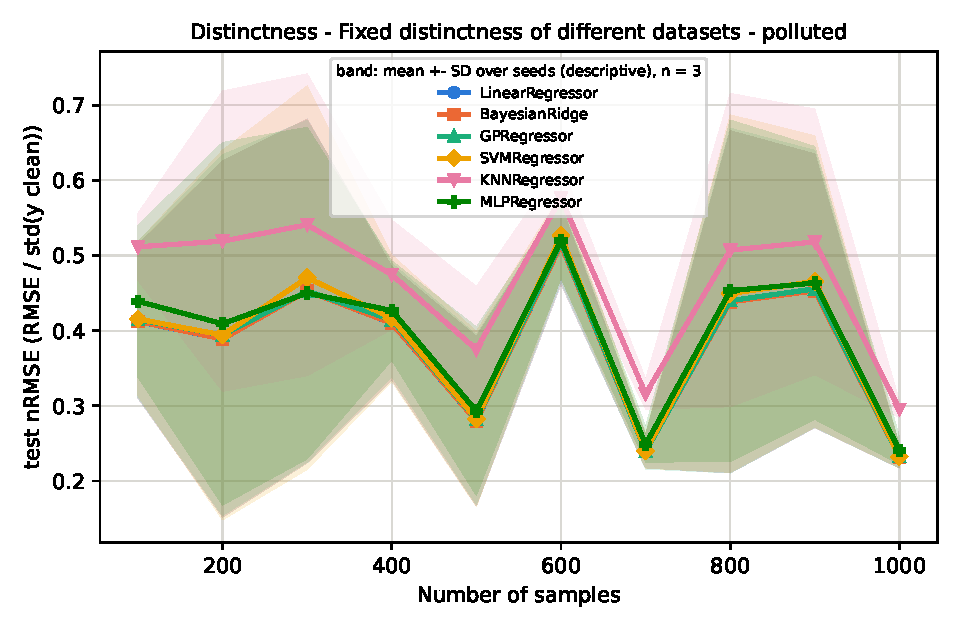
\includegraphics[width=0.8\textwidth]{v3/d3_fixed_n/polluted_test_nrmse.pdf}
\caption{D3: test nRMSE of each model, condition \texttt{polluted}, mean $\pm$ SD over 3 seeds.}
\label{fig:d3_fixed_n_polluted_test_nrmse}
\end{figure}

\begin{table}[htbp]
\centering
\small
\resizebox{\textwidth}{!}{% Generated by Report/tools/build_v3_assets.py from Plot/v3/results/d3_fixed_n.json (metric test_nrmse); do not edit by hand.
% Cells are mean $\pm$ SD over seeds (folds averaged within seed); the band is descriptive, not a confidence interval.
\begin{tabular}{llrrr}
\hline
Condition & Model & 100 & 600 & 1000 \\
\hline
polluted & LinearRegressor & 0.412 $\pm$ 0.102 & 0.514 $\pm$ 0.052 & 0.232 $\pm$ 0.015 \\
polluted & BayesianRidge & 0.412 $\pm$ 0.102 & 0.514 $\pm$ 0.052 & 0.232 $\pm$ 0.015 \\
polluted & GPRegressor & 0.415 $\pm$ 0.103 & 0.517 $\pm$ 0.052 & 0.233 $\pm$ 0.015 \\
polluted & SVMRegressor & 0.415 $\pm$ 0.102 & 0.526 $\pm$ 0.056 & 0.232 $\pm$ 0.015 \\
polluted & KNNRegressor & 0.512 $\pm$ 0.045 & 0.577 $\pm$ 0.045 & 0.295 $\pm$ 0.011 \\
polluted & MLPRegressor & 0.439 $\pm$ 0.101 & 0.520 $\pm$ 0.050 & 0.241 $\pm$ 0.018 \\
clean & LinearRegressor & 0.188 $\pm$ 0.015 & 0.197 $\pm$ 0.004 & 0.199 $\pm$ 0.004 \\
\hline
\end{tabular}
}
\caption{D3: test nRMSE (lower is better) against sample size $n$ (100, 600, 1000 shown); mean $\pm$ SD over 3 seeds.}
\label{tab:d3_fixed_n}
\end{table}

\subsection{D4: different percentages among features}
\label{sec:d4_features}
Several of 9 features (4 informative) are polluted with percentages drawn around $x$. The linear model gives $0.347 \pm 0.131$, $0.645 \pm 0.226$ and $0.756 \pm 0.231$ (clean $0.200$); \texttt{KNeighborsRegressor} gives $0.551$, $0.788$ and $0.869$. The SD over seeds is large because the set of polluted columns differs between seeds.

\begin{figure}[htbp]
\centering
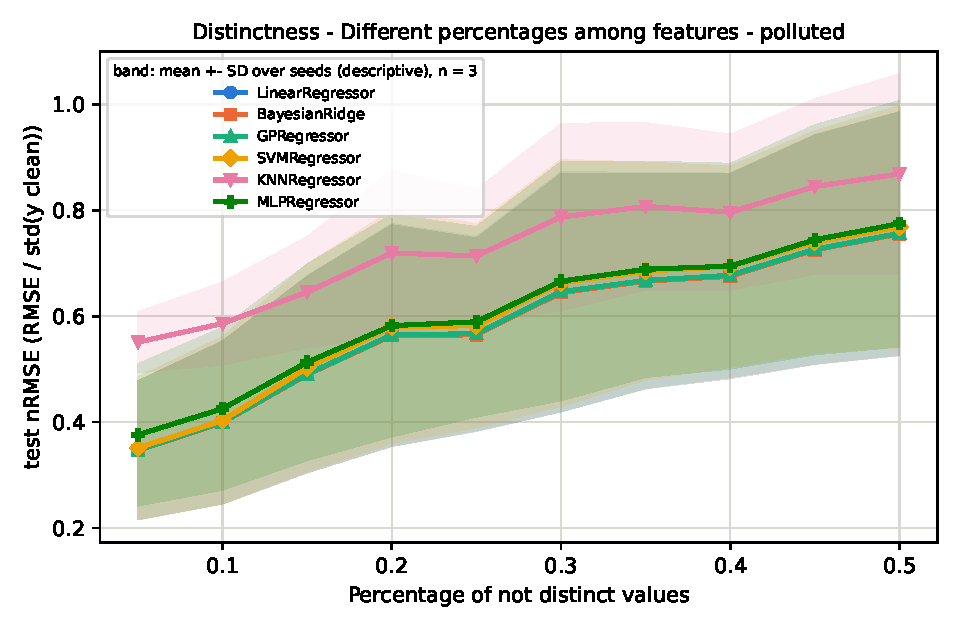
\includegraphics[width=0.8\textwidth]{v3/d4_features/polluted_test_nrmse.pdf}
\caption{D4: test nRMSE of each model, condition \texttt{polluted}, mean $\pm$ SD over 3 seeds.}
\label{fig:d4_features_polluted_test_nrmse}
\end{figure}

\begin{table}[htbp]
\centering
\small
\resizebox{\textwidth}{!}{% Generated by Report/tools/build_v3_assets.py from Plot/v3/results/d4_features.json (metric test_nrmse); do not edit by hand.
% Cells are mean $\pm$ SD over seeds (folds averaged within seed); the band is descriptive, not a confidence interval.
\begin{tabular}{llrrr}
\hline
Condition & Model & 0.05 & 0.3 & 0.5 \\
\hline
polluted & LinearRegressor & 0.347 $\pm$ 0.131 & 0.645 $\pm$ 0.226 & 0.756 $\pm$ 0.231 \\
polluted & BayesianRidge & 0.347 $\pm$ 0.131 & 0.644 $\pm$ 0.225 & 0.755 $\pm$ 0.230 \\
polluted & GPRegressor & 0.347 $\pm$ 0.132 & 0.646 $\pm$ 0.227 & 0.757 $\pm$ 0.230 \\
polluted & SVMRegressor & 0.351 $\pm$ 0.135 & 0.663 $\pm$ 0.234 & 0.769 $\pm$ 0.229 \\
polluted & KNNRegressor & 0.551 $\pm$ 0.058 & 0.788 $\pm$ 0.177 & 0.869 $\pm$ 0.189 \\
polluted & MLPRegressor & 0.376 $\pm$ 0.135 & 0.666 $\pm$ 0.226 & 0.775 $\pm$ 0.233 \\
clean & LinearRegressor & 0.200 $\pm$ 0.005 & 0.200 $\pm$ 0.005 & 0.200 $\pm$ 0.005 \\
\hline
\end{tabular}
}
\caption{D4: test nRMSE (lower is better) against mean percentage (0.05, 0.3, 0.5 shown); mean $\pm$ SD over 3 seeds.}
\label{tab:d4_features}
\end{table}

\subsection{D8: high and low distinctness combined}
\label{sec:d8_high_low}
Two random columns are polluted, with $x$ and $1-x$ non-distinct values. At $x=0.25$ the linear model is at $0.865 \pm 0.081$ and at 50\% at $0.911 \pm 0.034$, close to the nRMSE of 1 of a mean predictor; \texttt{KNeighborsRegressor} reaches $0.948$ and $0.986$.

\begin{figure}[htbp]
\centering
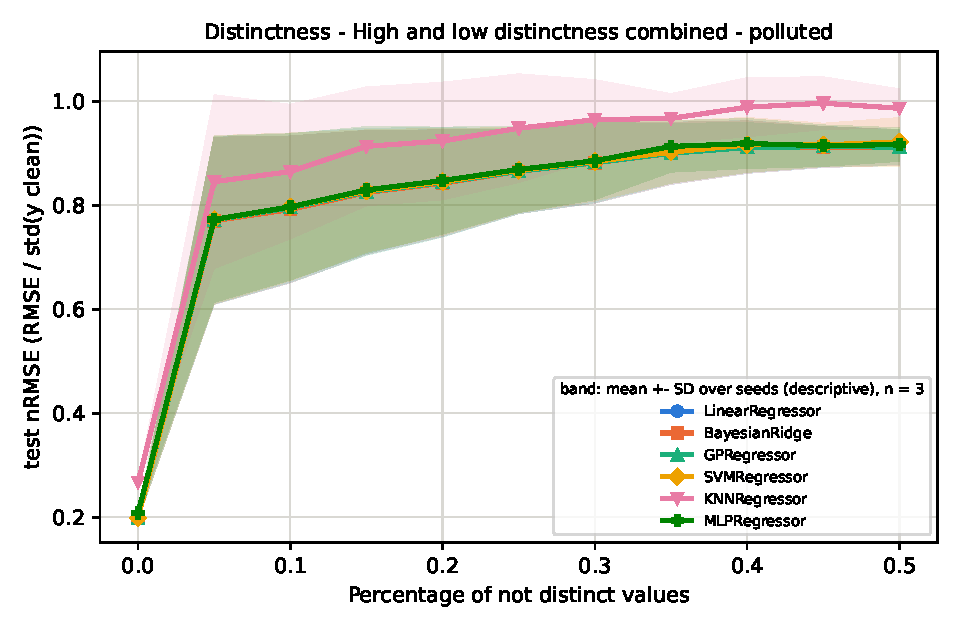
\includegraphics[width=0.8\textwidth]{v3/d8_high_low/polluted_test_nrmse.pdf}
\caption{D8: test nRMSE of each model, condition \texttt{polluted}, mean $\pm$ SD over 3 seeds.}
\label{fig:d8_high_low_polluted_test_nrmse}
\end{figure}

\begin{table}[htbp]
\centering
\small
\resizebox{\textwidth}{!}{% Generated by Report/tools/build_v3_assets.py from Plot/v3/results/d8_high_low.json (metric test_nrmse); do not edit by hand.
% Cells are mean $\pm$ SD over seeds (folds averaged within seed); the band is descriptive, not a confidence interval.
\begin{tabular}{llrrr}
\hline
Condition & Model & 0 & 0.25 & 0.5 \\
\hline
polluted & LinearRegressor & 0.199 $\pm$ 0.004 & 0.865 $\pm$ 0.081 & 0.911 $\pm$ 0.034 \\
polluted & BayesianRidge & 0.199 $\pm$ 0.004 & 0.865 $\pm$ 0.081 & 0.911 $\pm$ 0.034 \\
polluted & GPRegressor & 0.199 $\pm$ 0.004 & 0.865 $\pm$ 0.082 & 0.912 $\pm$ 0.034 \\
polluted & SVMRegressor & 0.199 $\pm$ 0.004 & 0.867 $\pm$ 0.081 & 0.922 $\pm$ 0.047 \\
polluted & KNNRegressor & 0.267 $\pm$ 0.005 & 0.948 $\pm$ 0.105 & 0.986 $\pm$ 0.037 \\
polluted & MLPRegressor & 0.208 $\pm$ 0.005 & 0.869 $\pm$ 0.083 & 0.917 $\pm$ 0.032 \\
clean & LinearRegressor & 0.199 $\pm$ 0.004 & 0.199 $\pm$ 0.004 & 0.199 $\pm$ 0.004 \\
\hline
\end{tabular}
}
\caption{D8: test nRMSE (lower is better) against fraction of non-distinct values $x$ (0, 0.25, 0.5 shown); mean $\pm$ SD over 3 seeds.}
\label{tab:d8_high_low}
\end{table}

\subsection{D9: distinctness on the most informative features}
\label{sec:d9_informative}
The 3 most important of 9 features are polluted. The linear model goes from $0.200$ to $0.698 \pm 0.029$ and $0.918 \pm 0.025$, and \texttt{KNeighborsRegressor} from $0.471$ to $0.816$ and $1.019 \pm 0.015$, i.e. worse than a mean predictor.

\begin{figure}[htbp]
\centering
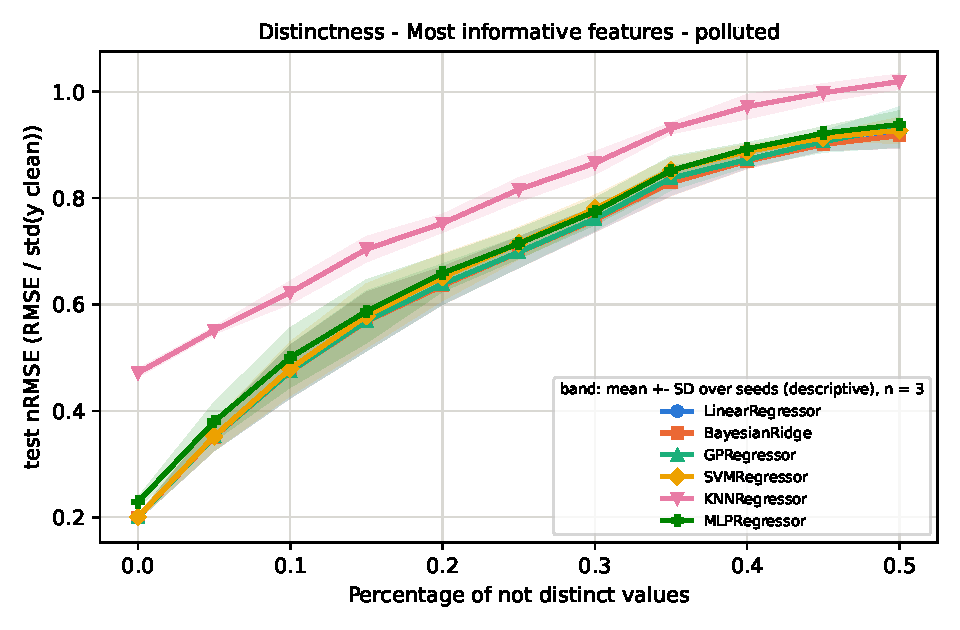
\includegraphics[width=0.8\textwidth]{v3/d9_informative/polluted_test_nrmse.pdf}
\caption{D9: test nRMSE of each model, condition \texttt{polluted}, mean $\pm$ SD over 3 seeds.}
\label{fig:d9_informative_polluted_test_nrmse}
\end{figure}

\begin{table}[htbp]
\centering
\small
\resizebox{\textwidth}{!}{% Generated by Report/tools/build_v3_assets.py from Plot/v3/results/d9_informative.json (metric test_nrmse); do not edit by hand.
% Cells are mean $\pm$ SD over seeds (folds averaged within seed); the band is descriptive, not a confidence interval.
\begin{tabular}{llrrr}
\hline
Condition & Model & 0 & 0.25 & 0.5 \\
\hline
polluted & LinearRegressor & 0.200 $\pm$ 0.005 & 0.698 $\pm$ 0.029 & 0.918 $\pm$ 0.025 \\
polluted & BayesianRidge & 0.200 $\pm$ 0.005 & 0.698 $\pm$ 0.029 & 0.918 $\pm$ 0.024 \\
polluted & GPRegressor & 0.200 $\pm$ 0.005 & 0.698 $\pm$ 0.029 & 0.934 $\pm$ 0.038 \\
polluted & SVMRegressor & 0.201 $\pm$ 0.004 & 0.715 $\pm$ 0.030 & 0.927 $\pm$ 0.025 \\
polluted & KNNRegressor & 0.471 $\pm$ 0.008 & 0.816 $\pm$ 0.023 & 1.019 $\pm$ 0.015 \\
polluted & MLPRegressor & 0.228 $\pm$ 0.009 & 0.714 $\pm$ 0.028 & 0.939 $\pm$ 0.026 \\
clean & LinearRegressor & 0.200 $\pm$ 0.005 & 0.200 $\pm$ 0.005 & 0.200 $\pm$ 0.005 \\
\hline
\end{tabular}
}
\caption{D9: test nRMSE (lower is better) against fraction of non-distinct values (0, 0.25, 0.5 shown); mean $\pm$ SD over 3 seeds.}
\label{tab:d9_informative}
\end{table}

\subsection{D10: distinctness on the less informative features}
\label{sec:d10_less_informative}
The same on the 3 least important features. The linear model stays at $0.200$, $0.200$, $0.199$, equal to the clean reference, and so do BayesianRidge, the Gaussian process and \texttt{LinearSVR} (about $0.20$). \texttt{KNeighborsRegressor} is high ($0.471$ at rate 0) but also essentially flat ($0.479$, $0.482$): its level comes from the many uninformative columns that enter the distance, not from the pollution. This contradicts the original statement that the pollution of unimportant features was crucial.

\begin{figure}[htbp]
\centering
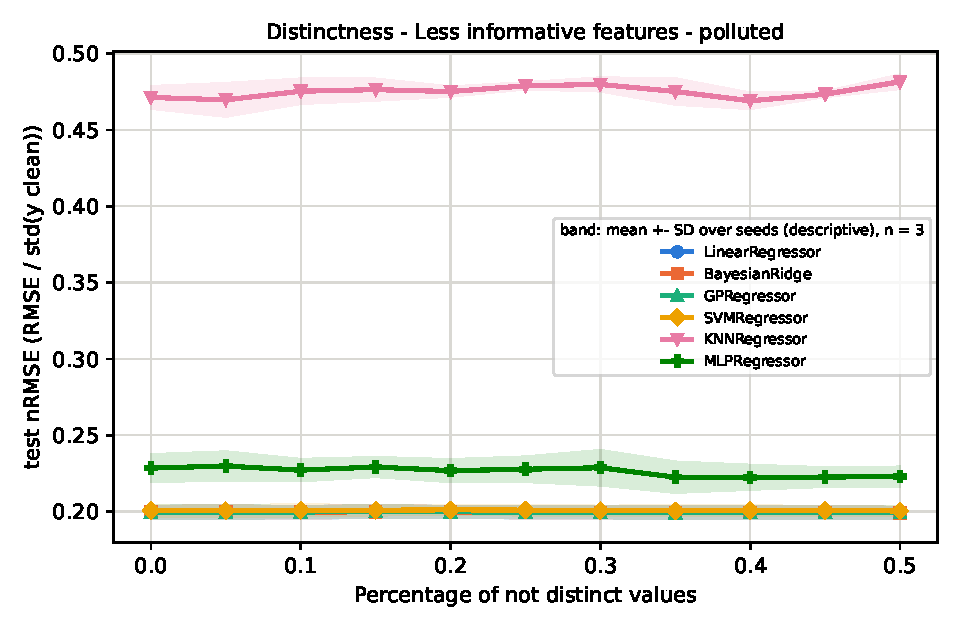
\includegraphics[width=0.8\textwidth]{v3/d10_less_informative/polluted_test_nrmse.pdf}
\caption{D10: test nRMSE of each model, condition \texttt{polluted}, mean $\pm$ SD over 3 seeds.}
\label{fig:d10_less_informative_polluted_test_nrmse}
\end{figure}

\begin{table}[htbp]
\centering
\small
\resizebox{\textwidth}{!}{% Generated by Report/tools/build_v3_assets.py from Plot/v3/results/d10_less_informative.json (metric test_nrmse); do not edit by hand.
% Cells are mean $\pm$ SD over seeds (folds averaged within seed); the band is descriptive, not a confidence interval.
\begin{tabular}{llrrr}
\hline
Condition & Model & 0 & 0.25 & 0.5 \\
\hline
polluted & LinearRegressor & 0.200 $\pm$ 0.005 & 0.200 $\pm$ 0.004 & 0.199 $\pm$ 0.004 \\
polluted & BayesianRidge & 0.200 $\pm$ 0.005 & 0.200 $\pm$ 0.004 & 0.199 $\pm$ 0.004 \\
polluted & GPRegressor & 0.200 $\pm$ 0.005 & 0.200 $\pm$ 0.004 & 0.199 $\pm$ 0.004 \\
polluted & SVMRegressor & 0.201 $\pm$ 0.004 & 0.201 $\pm$ 0.004 & 0.200 $\pm$ 0.004 \\
polluted & KNNRegressor & 0.471 $\pm$ 0.008 & 0.479 $\pm$ 0.003 & 0.482 $\pm$ 0.005 \\
polluted & MLPRegressor & 0.228 $\pm$ 0.009 & 0.228 $\pm$ 0.009 & 0.223 $\pm$ 0.007 \\
clean & LinearRegressor & 0.200 $\pm$ 0.005 & 0.200 $\pm$ 0.005 & 0.200 $\pm$ 0.005 \\
\hline
\end{tabular}
}
\caption{D10: test nRMSE (lower is better) against fraction of non-distinct values (0, 0.25, 0.5 shown); mean $\pm$ SD over 3 seeds.}
\label{tab:d10_less_informative}
\end{table}

\subsection*{Family B: duplicate records}
\subsection{D11: duplicate records}
\label{sec:d11_duplicates}
Exact copies of rows are appended (1000 original rows, 3 features). With group-aware splits (\texttt{duplicated}) the linear model is unaffected ($0.199$ at all rates), and \texttt{KNeighborsRegressor} rises moderately from $0.267$ to $0.274 \pm 0.004$ and $0.283 \pm 0.006$ because copies re-weight neighbours. Deduplicating the training fold removes this effect ($0.267$ throughout). With the leaky \texttt{naive\_split} the linear model is still unchanged, but \texttt{KNeighborsRegressor} appears to improve from $0.267$ to $0.251 \pm 0.002$ and $0.223 \pm 0.002$ because copies of training rows are scored in the test fold: an optimistic, invalid estimate.

\begin{figure}[htbp]
\centering
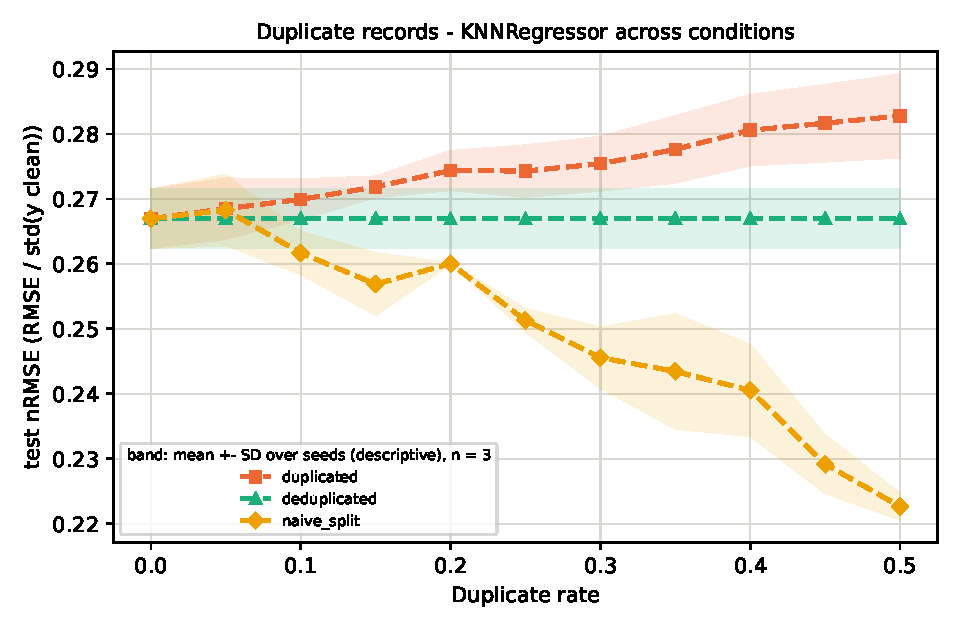
\includegraphics[width=0.8\textwidth]{v3/d11_duplicates/model_KNNRegressor_test_nrmse.pdf}
\caption{D11: test nRMSE of \texttt{KNNRegressor} for each condition, mean $\pm$ SD over 3 seeds.}
\label{fig:d11_duplicates_model_KNNRegressor_test_nrmse}
\end{figure}

\begin{figure}[htbp]
\centering
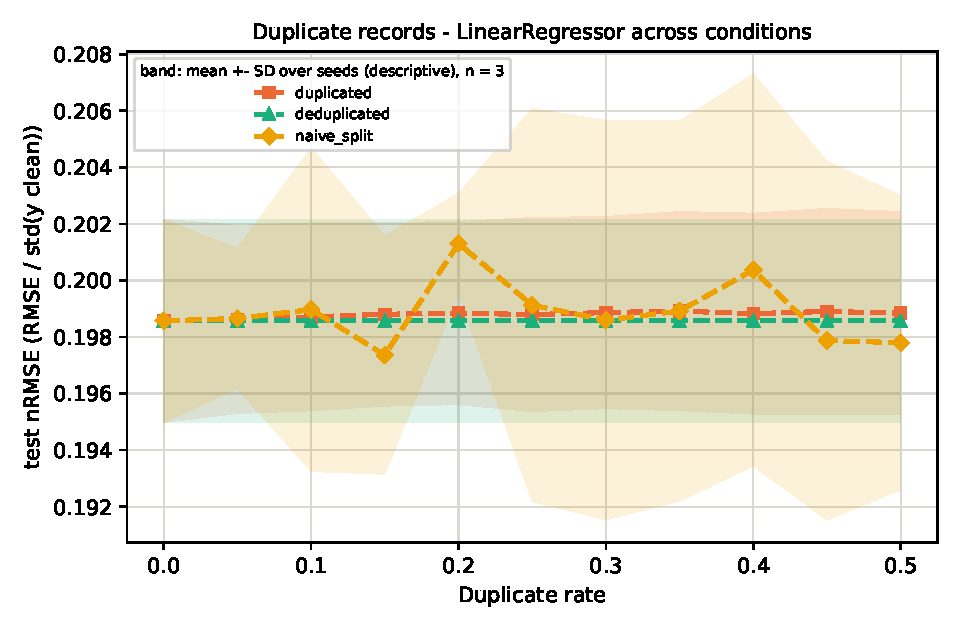
\includegraphics[width=0.8\textwidth]{v3/d11_duplicates/model_LinearRegressor_test_nrmse.pdf}
\caption{D11: test nRMSE of \texttt{LinearRegressor} for each condition, mean $\pm$ SD over 3 seeds.}
\label{fig:d11_duplicates_model_LinearRegressor_test_nrmse}
\end{figure}

\begin{table}[htbp]
\centering
\small
\resizebox{\textwidth}{!}{% Generated by Report/tools/build_v3_assets.py from Plot/v3/results/d11_duplicates.json (metric test_nrmse); do not edit by hand.
% Cells are mean $\pm$ SD over seeds (folds averaged within seed); the band is descriptive, not a confidence interval.
\begin{tabular}{llrrr}
\hline
Condition & Model & 0 & 0.25 & 0.5 \\
\hline
duplicated & LinearRegressor & 0.199 $\pm$ 0.004 & 0.199 $\pm$ 0.003 & 0.199 $\pm$ 0.004 \\
duplicated & KNNRegressor & 0.267 $\pm$ 0.005 & 0.274 $\pm$ 0.004 & 0.283 $\pm$ 0.006 \\
deduplicated & LinearRegressor & 0.199 $\pm$ 0.004 & 0.199 $\pm$ 0.004 & 0.199 $\pm$ 0.004 \\
deduplicated & KNNRegressor & 0.267 $\pm$ 0.005 & 0.267 $\pm$ 0.005 & 0.267 $\pm$ 0.005 \\
naive\_split & LinearRegressor & 0.199 $\pm$ 0.004 & 0.199 $\pm$ 0.007 & 0.198 $\pm$ 0.005 \\
naive\_split & KNNRegressor & 0.267 $\pm$ 0.005 & 0.251 $\pm$ 0.002 & 0.223 $\pm$ 0.002 \\
\hline
\end{tabular}
}
\caption{D11: test nRMSE (lower is better) against duplicate rate (0, 0.25, 0.5 shown); mean $\pm$ SD over 3 seeds.}
\label{tab:d11_duplicates}
\end{table}

\subsection*{Family C: accuracy and validity}
\subsection{D5: random noise on the features (accuracy)}
\label{sec:d5_noise}
Gaussian noise is added to all cells. The linear model degrades smoothly, $0.216 \pm 0.005$, $0.279 \pm 0.008$ and $0.318 \pm 0.010$ (clean $0.199$), all models by almost the same amount (\texttt{KNeighborsRegressor} $0.282$, $0.337$, $0.377$). This is the usual attenuation by errors in the features.

\begin{figure}[htbp]
\centering
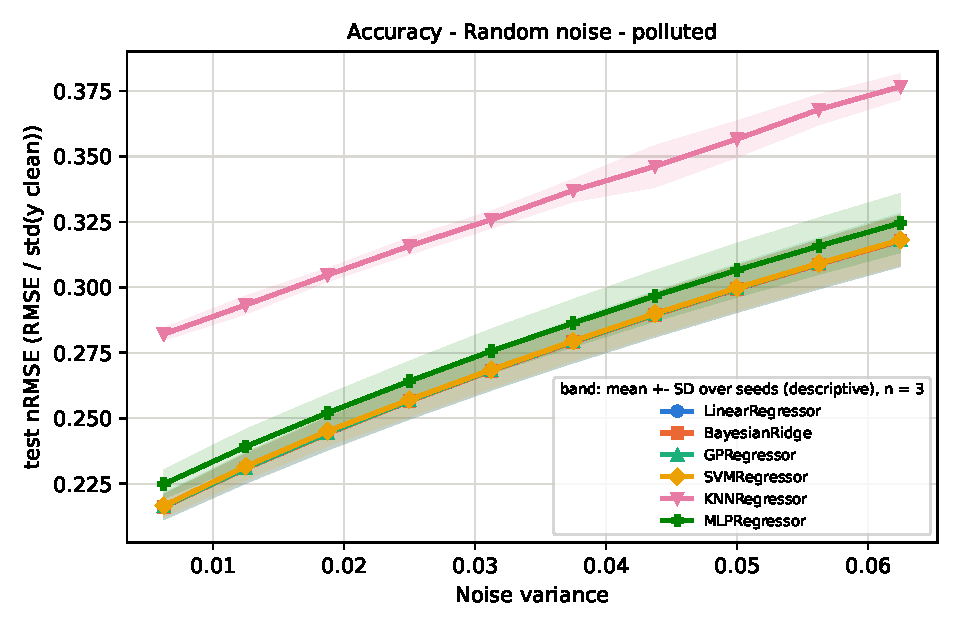
\includegraphics[width=0.8\textwidth]{v3/d5_noise/polluted_test_nrmse.pdf}
\caption{D5: test nRMSE of each model, condition \texttt{polluted}, mean $\pm$ SD over 3 seeds.}
\label{fig:d5_noise_polluted_test_nrmse}
\end{figure}

\begin{table}[htbp]
\centering
\small
\resizebox{\textwidth}{!}{% Generated by Report/tools/build_v3_assets.py from Plot/v3/results/d5_noise.json (metric test_nrmse); do not edit by hand.
% Cells are mean $\pm$ SD over seeds (folds averaged within seed); the band is descriptive, not a confidence interval.
\begin{tabular}{llrrr}
\hline
Condition & Model & 0.00625 & 0.0375 & 0.0625 \\
\hline
polluted & LinearRegressor & 0.216 $\pm$ 0.005 & 0.279 $\pm$ 0.008 & 0.318 $\pm$ 0.010 \\
polluted & BayesianRidge & 0.216 $\pm$ 0.005 & 0.279 $\pm$ 0.008 & 0.318 $\pm$ 0.010 \\
polluted & GPRegressor & 0.216 $\pm$ 0.005 & 0.279 $\pm$ 0.008 & 0.318 $\pm$ 0.010 \\
polluted & SVMRegressor & 0.217 $\pm$ 0.004 & 0.279 $\pm$ 0.008 & 0.318 $\pm$ 0.010 \\
polluted & KNNRegressor & 0.282 $\pm$ 0.002 & 0.337 $\pm$ 0.004 & 0.377 $\pm$ 0.005 \\
polluted & MLPRegressor & 0.225 $\pm$ 0.006 & 0.286 $\pm$ 0.009 & 0.325 $\pm$ 0.011 \\
clean & LinearRegressor & 0.199 $\pm$ 0.004 & 0.199 $\pm$ 0.004 & 0.199 $\pm$ 0.004 \\
\hline
\end{tabular}
}
\caption{D5: test nRMSE (lower is better) against noise variance (0.00625, 0.0375, 0.0625 shown); mean $\pm$ SD over 3 seeds.}
\label{tab:d5_noise}
\end{table}

\subsection{D6: binning one feature (precision)}
\label{sec:d6_bins}
With 1 bin the feature is constant and the linear model is at $0.630 \pm 0.233$; with 6 bins it recovers to $0.265 \pm 0.044$ and with 10 bins to $0.229 \pm 0.019$, still above the clean $0.199$. Binning always loses information; the apparent improvement with more bins is the recovery of that information, not a benefit of discretisation.

\begin{figure}[htbp]
\centering
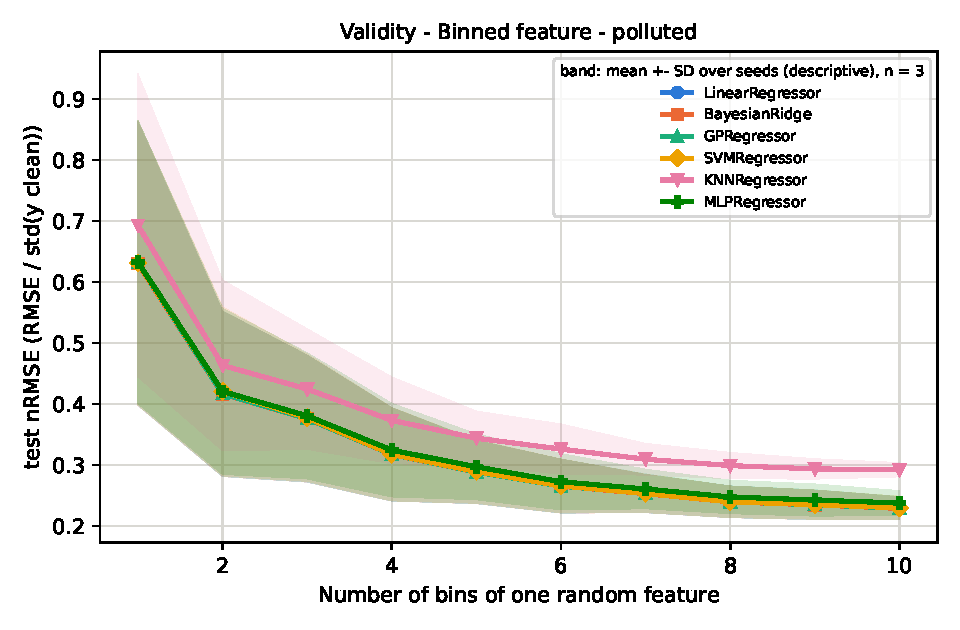
\includegraphics[width=0.8\textwidth]{v3/d6_bins/polluted_test_nrmse.pdf}
\caption{D6: test nRMSE of each model, condition \texttt{polluted}, mean $\pm$ SD over 3 seeds.}
\label{fig:d6_bins_polluted_test_nrmse}
\end{figure}

\begin{table}[htbp]
\centering
\small
\resizebox{\textwidth}{!}{% Generated by Report/tools/build_v3_assets.py from Plot/v3/results/d6_bins.json (metric test_nrmse); do not edit by hand.
% Cells are mean $\pm$ SD over seeds (folds averaged within seed); the band is descriptive, not a confidence interval.
\begin{tabular}{llrrr}
\hline
Condition & Model & 1 & 6 & 10 \\
\hline
polluted & LinearRegressor & 0.630 $\pm$ 0.233 & 0.265 $\pm$ 0.044 & 0.229 $\pm$ 0.019 \\
polluted & BayesianRidge & 0.630 $\pm$ 0.233 & 0.265 $\pm$ 0.044 & 0.229 $\pm$ 0.019 \\
polluted & GPRegressor & 0.632 $\pm$ 0.233 & 0.265 $\pm$ 0.044 & 0.229 $\pm$ 0.019 \\
polluted & SVMRegressor & 0.631 $\pm$ 0.233 & 0.266 $\pm$ 0.044 & 0.230 $\pm$ 0.019 \\
polluted & KNNRegressor & 0.693 $\pm$ 0.249 & 0.326 $\pm$ 0.041 & 0.292 $\pm$ 0.012 \\
polluted & MLPRegressor & 0.633 $\pm$ 0.232 & 0.272 $\pm$ 0.046 & 0.237 $\pm$ 0.020 \\
clean & LinearRegressor & 0.199 $\pm$ 0.004 & 0.199 $\pm$ 0.004 & 0.199 $\pm$ 0.004 \\
\hline
\end{tabular}
}
\caption{D6: test nRMSE (lower is better) against number of bins (1, 6, 10 shown); mean $\pm$ SD over 3 seeds.}
\label{tab:d6_bins}
\end{table}

\subsection{D7: outliers (validity)}
\label{sec:d7_outliers}
A random cell in the chosen rows is replaced by a random integer in $[0, 100)$, up to about 100 standard deviations of the Gaussian features, an extreme contamination. The linear model, BayesianRidge and \texttt{LinearSVR} fail: $1.256 \pm 0.305$, $0.992$ and $0.996$ for the linear model, $2.397 \pm 0.189$ at 1.25\% for \texttt{LinearSVR}, i.e. no better than (or worse than) a mean predictor. The Gaussian process ($0.242$, $0.376$, $0.452$) and \texttt{KNeighborsRegressor} ($0.315$, $0.399$, $0.479$) degrade gracefully, and the MLP lies in between ($0.527 \pm 0.229$, $0.337$, $0.399$).

\begin{figure}[htbp]
\centering
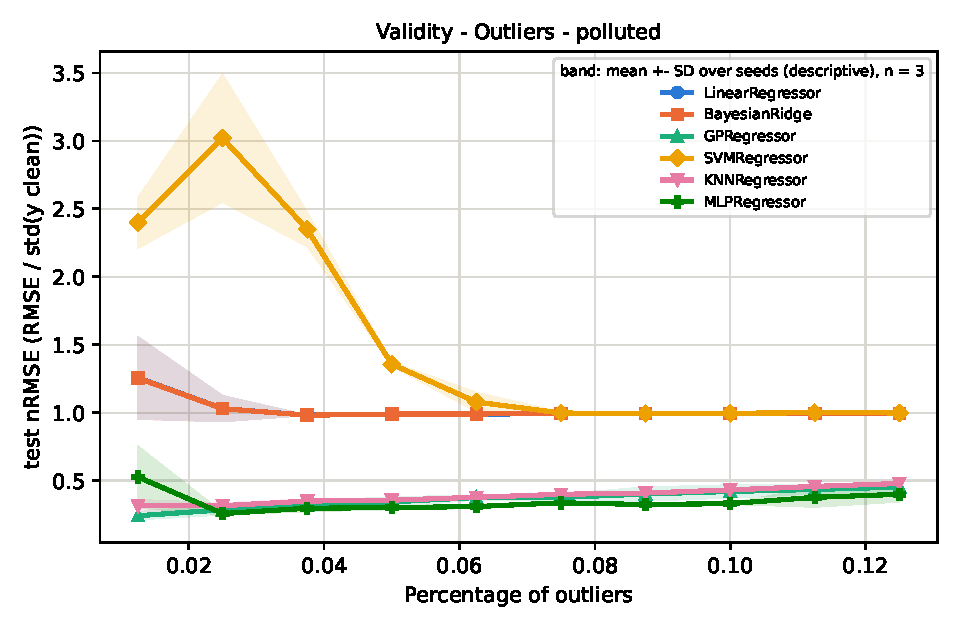
\includegraphics[width=0.8\textwidth]{v3/d7_outliers/polluted_test_nrmse.pdf}
\caption{D7: test nRMSE of each model, condition \texttt{polluted}, mean $\pm$ SD over 3 seeds.}
\label{fig:d7_outliers_polluted_test_nrmse}
\end{figure}

\begin{table}[htbp]
\centering
\small
\resizebox{\textwidth}{!}{% Generated by Report/tools/build_v3_assets.py from Plot/v3/results/d7_outliers.json (metric test_nrmse); do not edit by hand.
% Cells are mean $\pm$ SD over seeds (folds averaged within seed); the band is descriptive, not a confidence interval.
\begin{tabular}{llrrr}
\hline
Condition & Model & 0.0125 & 0.075 & 0.125 \\
\hline
polluted & LinearRegressor & 1.256 $\pm$ 0.305 & 0.992 $\pm$ 0.006 & 0.996 $\pm$ 0.004 \\
polluted & BayesianRidge & 1.254 $\pm$ 0.305 & 0.993 $\pm$ 0.007 & 0.996 $\pm$ 0.005 \\
polluted & GPRegressor & 0.242 $\pm$ 0.031 & 0.376 $\pm$ 0.027 & 0.452 $\pm$ 0.031 \\
polluted & SVMRegressor & 2.397 $\pm$ 0.189 & 0.997 $\pm$ 0.010 & 0.998 $\pm$ 0.002 \\
polluted & KNNRegressor & 0.315 $\pm$ 0.047 & 0.399 $\pm$ 0.007 & 0.479 $\pm$ 0.010 \\
polluted & MLPRegressor & 0.527 $\pm$ 0.229 & 0.337 $\pm$ 0.015 & 0.399 $\pm$ 0.057 \\
clean & LinearRegressor & 0.199 $\pm$ 0.004 & 0.199 $\pm$ 0.004 & 0.199 $\pm$ 0.004 \\
\hline
\end{tabular}
}
\caption{D7: test nRMSE (lower is better) against fraction of rows with an outlier (0.0125, 0.075, 0.125 shown); mean $\pm$ SD over 3 seeds.}
\label{tab:d7_outliers}
\end{table}

\chapter{Conclusions and limitations}
\label{ch:chapter_5}%

\section{Conclusions}
\label{sec:conclusions}%
\begin{itemize}
    \item \textbf{MCAR.} Mean, median, iterative and mean-plus-indicator imputation are equivalent because the features are independent and the other columns carry no information about the missing one (\Cref{tab:c01_mcar_low,tab:c02_mcar_high}). \texttt{most\_frequent} is degenerate, \texttt{std\_constant} is clearly worse, and \texttt{knn} is slightly worse. The error grows steadily with the missing rate.
    \item \textbf{Only informative features matter.} Missing values in noise features leave the error at the clean level (C3 rank 5 and 9, C8), while the same rate in informative features is costly (C3 rank 0, C7, C9). D10 shows the same for distinctness.
    \item \textbf{MAR} is mild at the rates tested (\Cref{tab:c05_mar}), though only one column is affected so this is not like-for-like with MCAR on all features, with a large spread between seeds.
    \item \textbf{MNAR.} Mean and iterative imputation are biased; the missing-value indicator recovers a large part of the loss and the native boosting model behaves similarly (\Cref{tab:c06_mnar}). In the combined MCAR plus MNAR setting the advantage of the indicator disappears at high rates (\Cref{tab:c10_mcar_mnar}).
    \item \textbf{Duplicates} do not hurt the linear model with group-aware splits; \texttt{KNeighborsRegressor} is slightly affected and deduplication of the training fold removes the effect, while a naive split inflates the apparent performance of \texttt{KNeighborsRegressor} (\Cref{tab:d11_duplicates}).
    \item \textbf{Outliers} break the linear model, BayesianRidge and \texttt{LinearSVR}, which fall to or below the level of a mean predictor, while the Gaussian process and \texttt{KNeighborsRegressor} are more robust (\Cref{tab:d7_outliers}). Noise and binning degrade all models smoothly (D5, D6).
    \item \textbf{Substitution.} Pasting a value into a column behaves as an accuracy error: the effect scales with feature importance and saturates (D1, D2; D8 is near the ceiling).
    \item \textbf{Sample size.} The sample-size experiments with pollution (C4, D3) show no consistent size trend (C4 with a large seed variance, D3 with variation between $n$ values that reflects the weight of the polluted feature, which changes with $n$ because the data are regenerated); only the clean learning curve (C0) shows a size effect, mainly for \texttt{KNeighborsRegressor}.
\end{itemize}

\section{Limitations}
\label{sec:limitations}%
\begin{itemize}
    \item Only 3 seeds are used, so the SD is a rough descriptive spread and not a confidence interval.
    \item The data are synthetic with independent Gaussian features; the conclusion that simple imputers are equivalent depends on this and would not hold for correlated features.
    \item \texttt{MLPRegressor} and \texttt{LinearSVR} may report convergence warnings, which are recorded in the fold status and not suppressed.
    \item In C9 the groups of features share row sets with C7, and in C4 the missing-row sets of the columns are nested.
    \item The figures and tables are generated from the saved results (\texttt{Plot/v3}) by \texttt{Report/tools/build\_v3\_assets.py}; they are only as current as the last notebook run.
    \item The tables show three points of each x axis; the complete series are in the figures and in the results files.
\end{itemize}

\cleardoublepage
\begin{thebibliography}{100}
        \bibitem{github_reference} \textbf{GitHub repository that contains all the experiments mentioned in the document} \href{https://github.com/BiancaSavoiu/DIQ_project}{https://github.com/BiancaSavoiu/DIQproject}
        \bibitem{rubin1976} D.~B. Rubin. Inference and missing data. \textit{Biometrika}, 63(3):581--592, 1976.
        \bibitem{littlerubin2019} R.~J.~A. Little and D.~B. Rubin. \textit{Statistical Analysis with Missing Data}, 3rd edition. Wiley, 2019.
        \bibitem{josse2019} J.~Josse, N.~Prost, E.~Scornet and G.~Varoquaux. On the consistency of supervised learning with missing values. arXiv:1902.06931, 2019.
        \bibitem{batini2016} C.~Batini and M.~Scannapieco. \textit{Data and Information Quality}. Springer, 2016.
        \bibitem{pedregosa2011} F.~Pedregosa et al. Scikit-learn: Machine learning in Python. \textit{Journal of Machine Learning Research}, 12:2825--2830, 2011.
        \bibitem{rasmussen2006} C.~E. Rasmussen and C.~K.~I. Williams. \textit{Gaussian Processes for Machine Learning}. MIT Press, 2006.
        \bibitem{kaufman2012} S.~Kaufman, S.~Rosset, C.~Perlich and O.~Stitelman. Leakage in data mining. \textit{ACM Transactions on Knowledge Discovery from Data}, 6(4), 2012.
    \end{thebibliography}
\end{document}
